% *****************************************************************************
%     sections/chapter1.tex
%
% Last edit: 05/03
% *****************************************************************************

\chapter{Structure and equation of state of cold non-accreting neutron stars}

This chapter deals with the structure and equation of state (EoS) of neutron 
stars (NS) within the framework of the ``cold catalyzed matter'' 
(CCM) hypothesis.

With typical temperature of about $T \sim 10^8$ K $\sim 0.01$ MeV$/k_B$, NS are 
very cold systems from the nuclear physics viewpoint, therefore the CCM hypothesis 
is commonly used to predict their internal composition and pressure. In this 
limit, thermal, nuclear, and beta equilibrium are established at zero
temperature, meaning that the energy cannot be lowered by weak, strong, or 
electromagnetic processes, thus the matter is in its ground state. It is 
reasonable to expect these equilibrium conditions to be valid in any NS as far 
as it is not accreting matter from a neighbor. Indeed, in the accretion 
scenario, the typical timescale of the process are such that the matter
composition is believed to be out of equilibrium.

As already discussed in the general introduction, the EoS 
relates, in given conditions of temperature and densities, the macroscopic
quantities of the star, such as the mass density and the pressure, which
determines among others the mass-radius relation of NS. The evaluation of the
EoS therefore implies to know the microscopic composition at each point in the
star. At subsaturation densities, the solid crust consists mainly of 
clusterized matter, arranged in a body-centered cubic lattice~\cite{Haensel2007}. 
The relevant degrees of freedom in the crust are the Wigner-Seitz (WS) 
cells, containing exactly one lattice point \cite{Wigner1933}. At zero
temperature, WS cells are supposed to be identical, thus the so-called single
nucleus approximation (SNA), which considers a unique configuration for a given 
thermodynamic condition of temperature and pressure $(P,T)$, becomes exact. The 
ground state of the outer crust is almost entirely characterized by experimental 
nuclear masses, which are available up to $(N-Z)/A \lesssim 0.3$. The 
determination of inner-crust ground state is however more challenging because 
the crust is permeated by free neutrons, a situation which cannot be achieved
in terrestrial conditions. Therefore, different treatments, from 
microscopic \cite{Negele1973} to classical~\cite{BBP}, can be envisaged to
estimate the energy of matter, and the EoS in this region depends on the 
nucleon-nucleon (NN) effective interaction or energy functional. At 
suprasaturation densities, matter consists of a uniform plasma of neutrons, 
protons, electrons, and eventually muons, in both strong and weak equilibrium. 
The development of a unified EoS, that is such that 
matter at subsaturation and supersaturation densities are treated within a
unique model, is essential if one wants to make realistic predictions on NS
observables~\cite{Fortin2016}.

The plan of the chapter is as follows. In Section~\ref{sec:ocrust_gs}, the 
ground state of the outer crust is determined by application of the 
method introduced by Baym, Pethick, and Sutherland (BPS)~\cite{BPS}, using 
experimental masses~\cite{Huang2017} supplemented by 
state-of-the-art microscopic theoretical mass tables. 
Section \ref{sec:icrust_gs} is devoted to the determination of the inner-crust ground 
state using a compressible liquid drop model (CLDM) based on the metamodeling
technique \cite{Margueron2018a,Carreau2019cc}. The phase transition 
from the solid crust to the liquid core, occuring at some $\approx 1$ km from the 
surface of the star, is investigated. In Section~\ref{sec:core}, we calculate 
the ground state of matter in the outer core, and we address the problem of the 
inner-core composition. In Section~\ref{sec:mmeos}, a unified metamodeling of 
the EoS is proposed. Finally, conclusions are given in Section~\ref{sec:conclu1}.

\minitoc\newpage

\section{Ground state of the outer crust}\label{sec:ocrust_gs}

At zero temperature, the matter inside the outer crust corresponds to a 
lattice of strongly bound nuclei, immersed in an sea of electrons. The mass 
density at which nuclei are fully ionized and electron completely degenerated 
is of the order of $\rho \gg 6AZ \sim 10^4$ g/cm$^3$ for $^{56}$Fe, which is
the ground state of matter at very low density. Below $10^4$ g/cm$^3$, some 
electrons are still bound to the nuclei and one must rely on the EoS 
calculated by Feynman, Metropolis, and Teller from 15 to $10^4$ g/cm$^3$, 
suitable for the envelope of neutron stars~\cite{Feynman1949}.

This section deals with the determination of the outer-crust ground state. 
In \ref{subsec:ws}, we detail the different terms entering in the WS cell 
energy, with emphasis on the relativistic electron gas energy as well as 
nuclear masses. The ground state of the outer crust is calculated by
application of the variational BPS method \cite{BPS}, which is 
presented in \ref{subsec:bps}. Finally, using current knowledge on experimental
masses~\cite{Huang2017} supplemented by different microscopic theoretical mass
tables, we compute the equilibrium composition and EoS. Our results are
presented in~\ref{subsec:ocrust_compo}.

\subsection{Wigner-Seitz cell energetics}\label{subsec:ws}

In the outer crust, a WS cell is composed of a strongly bound nucleus at the 
center, immersed in a relativistic electron gas of 
density $n_e$. Charge neutrality is assured in each unit cell, 
$n_e = n_p$, with $n_p$ the proton density inside the cell.

The energy of a WS cell in the outer crust can therefore be written as
%
\begin{equation}
  E_{WS} = E_i + V_{WS}\varepsilon_e,\label{eq:ews_ocrust}
\end{equation}
%
with $E_i$ the ion energy, $V_{WS}$ the volume of the cell, and $\varepsilon_e$ the 
energy density of the relativistic electron gas.
The ion energy reads
%
\begin{equation}
  E_i = M'(A,Z)c^2 + E_L + E_{zp},\label{eq:eion}
\end{equation}
%
where $M'(A,Z)c^2$ is the nuclear mass of a nucleus with associated mass number 
$A$ and charge number $Z$, $E_L$ the temperature-independent static-lattice 
term, and $E_{zp}$ the zero-point quantum vibration term given by
%
\begin{equation}
  E_{zp} = \frac{3}{2}\hbar \omega_p u_1,\label{eq:ezp}
\end{equation}
%
where $u_1 = 0.5113875$ is a numerical constant for a body-centered cubic
lattice (see Table 2.4 of~\cite{Haensel2007}), 
which is assumed to be the geometry minimizing the lattice energy. This
assumption was recently confirmed in~\cite{Chamel2016}. The ion
plasma frequency $\omega_p$ is given by
%
\begin{equation}
  \hbar \omega_p = \sqrt{\frac{(\hbar c)^2 4\pi n_N
  (Ze)^2}{M'(A,Z)c^2}},\label{eq:omegap}
\end{equation}
%
$e$ being the elementary charge, $c$ the speed of light, $\hbar = h/2\pi$
the reduced Planck constant, and where the ion density $n_N = 1/V_{WS}$ has
been introduced.\\
The lattice energy reads
%
\begin{equation}
  E_L = -C_M \frac{(Ze)^2}{a_N},\label{eq:eL}
\end{equation}
%
with $C_M = 0.895929255682$ the Mandelung constant for a body-centered cubic 
lattice (see Table 2.4 of~\cite{Haensel2007}), and $a_N = (4\pi n_N/3)^{-1/3}$ 
the ion-sphere radius.

\subsubsection{Nuclear mass tables}

An essential input for Eq.~(\ref{eq:eion}) is the nuclear mass table. When
available, that is for $I = (N-Z)/A \lesssim 0.3$, we use experimental masses
from the 2016 Atomic Mass Evaluation (AME)~\cite{Huang2017}. For more neutron-rich
nuclei and until we reach the neutron drip line, the use of a model is
required, thus a model dependence arises. A possibility is to rely on 
microscopic Hartree-Fock-Bogoliubov (HFB) theoretical mass
tables~\cite{Samyn2002}, which are based on the nuclear energy-density 
functional theory that is discussed in the general introduction.

In general, atomic masses are tabulated instead of the nuclear ones which can 
be calculated as
%
\begin{equation}
  M'(A,Z)c^2 = M(A,Z)c^2 - Zm_ec^2 + B_{e}(Z),
\end{equation}
%
with $M(A,Z)c^2 = \Delta \epsilon + Am_uc^2$ the atomic mass ($\Delta \epsilon$
is the mass excess, $m_u$ is atomic mass unit), $m_e$ the electron mass, and 
$B_e$ the binding energy of atomic electrons depending solely on the 
number of protons $Z$ according to the approximation proposed
in~\cite{Lunney2003} (see their Eq.~(A4)),
%
\begin{equation}
  B_e(Z) = 1.44381\times 10^{-5}Z^{2.39} + 1.55468\times 10^{-12}Z^{5.35}.
\end{equation}

\subsubsection{Relativistic electron gas}\label{subsubsec:elgas}

In the outer crust, the mass densities are above $\sim 10^4$ g/cm$^3$ therefore 
the electrons are essentially free.\\
The expression of the energy density of a relativistic electron gas, with rest
mass energy, at zero temperature can be calculated as
%
\begin{eqnarray}
  \varepsilon_e(n_e) &=& \int_0^{k_e}\frac{k^2dk}{\pi^2}c\sqrt{\hbar^2k^2 +
  {m_e}^2c^2}\notag \\
   &=& \frac{P_r}{8\pi^2}\left[x_r (1+2{x_r}^2)\gamma_r -
   \ln(x_r + \gamma_r)\right],\label{eq:eel}
\end{eqnarray}
%
with $P_r = {m_e}^4c^5/\hbar^3$ the relativistic unit of the electron pressure, 
$x_r = \hbar k_e/(m_ec)$ the relativity parameter, and $\gamma_r =
\sqrt{1 + {x_r}^2}$. $k_e$ is the electron Fermi wave number given by
%
\begin{equation}
  k_e = (3\pi^2n_e)^{1/3}.
\end{equation}
%
The derivation of Eq.~(\ref{eq:eel}) is given in Appendix \ref{appendix:epse}.\\
Above $10^7$ g/cm$^3$, $x_r \gg 1$, thus electrons can be considered 
ultrarelativistic and Eq.~(\ref{eq:eel}) becomes
%
\begin{equation}
  \varepsilon_e(n_e) = \frac{3}{4}n_e m_e c^2 x_r.\label{eq:eeur}
\end{equation}
%
Taking the derivative of Eq.~(\ref{eq:eel}) with respect to the electron gas 
density yields the pressure,
%
\begin{eqnarray}
  P_e &=& -\frac{\partial (V_{WS}\varepsilon_e)}{\partial V_{WS}} = n_e\frac{\partial
  \varepsilon_e}{\partial n_e} - \varepsilon_e \notag\\
      &=& \frac{P_r}{8\pi^2}\left[x_r(1+2{x_r}^2)\gamma_r - \ln(x_r +
      \gamma_r)\right].\label{eq:pel}
\end{eqnarray}
%

The exchanges and correlation corrections are neglected since they are known 
to be small in comparison to the kinetic energy of relativistic electrons. The 
expression of the exchange correction to the free energy density for a strongly 
degenerate electron gas is given in~\cite{Haensel2007} (see their Eq.~(2.151)).
We have checked that the inclusion of these corrections does not modify the
results presented in this chapter.

\subsection{The BPS model}\label{subsec:bps}

The variational technique which is currently used to calculate the ground state 
of the outer crust was introduced by Baym, Pethick, and Sutherland 
in~\cite{BPS}.

The zero-temperature Gibbs free energy per nucleon is the quantity to be minimized at fixed 
pressure $P$ under the condition of charge neutrality $n_e = Zn_N$, until the 
neutron drip sets in, the condition for which is $\mu_n =
m_n c^2$, with $\mu_n$ the neutron chemical potential, and $m_n$ the neutron
mass.

The definition of the zero-temperature Gibbs free energy per nucleon is
%
\begin{equation}
  g = \frac{\varepsilon_{WS} + P}{n_B},
\end{equation}
%
where $\varepsilon_{WS} = E_{WS}/V_{WS}$ is the energy density of the WS cell, and $n_B$ is the
baryon density given by $n_B = n_NA = A/V_{WS}$.\\
We can calculate the pressure as
%
\begin{equation}
  P = {n_B}^2\frac{\partial (\varepsilon_{WS}/n_B)}{\partial n_B}\Bigr|_{Z,A},
\end{equation}
%
yielding, using Eq.~(\ref{eq:ews_ocrust}),
%
\begin{equation}
  P = P_e + \frac{1}{3}E_Ln_N + \frac{1}{2}E_{zp}n_N.\label{eq:eq_pres}
\end{equation}
%
Thus the expression of the zero-temperature Gibbs free energy per nucleon
can be rewritten as 
%
\begin{equation}
  g = \frac{M'(A,Z)c^2 + \frac{4}{3}E_L + \frac{1}{2}E_{zp} + Z\mu_e}{A},
\end{equation}
%
where $\mu_e$ is the electron chemical potential given by
%
\begin{equation}
  \mu_e = \frac{\partial \varepsilon_e}{\partial n_e}.
\end{equation}
%
Essentially, one fixes the pressure $P$, calculates for each nucleus $(A,Z)$ 
the electronic density by solving numerically Eq.~(\ref{eq:eq_pres}), then
constructs a table $(g,A,Z)$. The ground state of the outer crust at pressure
$P$ then corresponds to the nucleus associated to the minimum value of $g$.

As explained in~\cite{Pearson2018}, the neutron chemical potential can be
calculated through
%
\begin{equation}
  \mu_n = g,
\end{equation}
%
because the beta equilibrium equation $\mu_n = \mu_p + \mu_e$ holds throughout
the star.
Indeed, by exploiting the thermodynamic relation
%
\begin{equation}
  \mathcal{G} = \varepsilon + P = \mu_n n_n + \mu_p n_p + \mu_e n_e,
\end{equation}
%
together with the charge neutrality condition $n_e = n_p$, we obtain
%
\begin{equation}
  \mathcal{G} = \mu_n n_n + (\mu_e + \mu_p)n_p,
\end{equation}
%
where $\mathcal{G}$ is the zero-temperature Gibbs free energy density, and
$\mu_p$ the proton chemical potential. In the case where 
the chemical equilibrium is established, that is if weak processes are at the 
equilibrium, we finally get
%
\begin{equation}
  \mathcal{G} = \mu_n n_B.
\end{equation}

% reason to minimize a fixed pressure p instead of baryon density nb:
One should stress that while minimizing the zero-temperature Gibbs 
free energy per nucleon at fixed 
pressure is less practical than simply minimizing the total energy density at 
constant baryon density, it makes it easier to study the transitions between layers. 
The pressure increases continuously with increasing depth in the star, thus a 
discontinuity in the density is the signature of a transition from a layer 
$(A,Z)$ to another $(A',Z')$. Noting that the pressure in the outer crust is 
approximately equal to the pressure of the electron gas (the lattice and
zero-point terms contribute to less than $5\%$ to the total pressure in the
bottom layers of the outer crust), we know that $n_e = n_p$ is 
continuous across the transition thus
%
\begin{equation}
  \Delta n_B = n_B' - n_B \simeq n_p\left(\frac{A'}{Z'} - \frac{A}{Z}\right),
\end{equation}
%
and the fractional change in the baryon mass density results 
%
\begin{equation}
  \frac{\Delta \rho_B}{\rho_B} \simeq \frac{\Delta n_B}{n_B} 
  \simeq \frac{Z/A}{Z'/A'} - 1.
\end{equation}
%
For this reason, it is more convenient to have the pressure as the 
independent variable. In this way we avoid to make a Maxwell construction to 
estimate the pressure at which the transition from $(A,Z)$ to $(A',Z')$ occurs.

The BPS model is still widely used to determine the ground state of the outer 
crust. However, at that time the authors took the values of nuclear binding 
energy from the outdated phenomenological macroscopic model of Myers and 
Swiatecki~\cite{Myers1965}. Moreover, they did not take
into account the zero-point vibration energy, Eq.~(\ref{eq:ezp}). In the last decades,
considerable efforts have been made to measure nuclear masses near the neutron
drip line~\cite{Lunney2003}, as well as theoretical developments were achieved 
to construct microscopic mass tables~\cite{Samyn2002}. It is therefore 
important to reevaluate the ground state of the outer crust considering those 
experimental and theoretical advances. In this line, Haensel and Pichon studied 
the consequences of progress concerning the experimental determination of atomic 
masses in 1994~\cite{Haensel1994}. The authors found that the ground state of
the outer crust can be determined exclusively by experimental masses in a fully
model independent way up to $\rho_B \approx 10^{11}$ g/cm$^3$. From this 
density up to the neutron drip point, the phenomenological, liquid-drop based 
mass formula of M\"oller was used, the formalism of which is described 
in~\cite{Moller1988}.

In the same spirit as~\cite{Haensel1994}, we calculate, in the following, the
ground state of the outer crust using the present day knowledge on experimental
masses of neutron rich nuclei~\cite{Huang2017,Welker2017} combined with 
state-of-the-art microscopic theoretical mass tables~\cite{Goriely2013}.

\subsection{Equilibrium composition and equation of state}\label{subsec:ocrust_compo}

We turn to the numerical results obtained applying the BPS method presented
in~\ref{subsec:bps}. The ground state of the outer crust is calculated,
beginning at $P = 3\times 10^{-11}$, corresponding approximately to 
$n_B \approx 10^{-9}$ fm$^{-3}$, in order to ensure complete ionization and 
electron degeneracy. The pressure is increased from steps of $0.02P$ until the 
neutron drip point, defined by $\mu_n - m_n c^2 = 0$, is reached.

\begin{table}[!t]
\begin{center}
\begin{tabular}{cccccccc} 
  \toprule
  \toprule
  element   & $Z$ & $N$ & $Y_p$  & $n_{B,max}$       & $P_{max}$    & $\mu_n - m_nc^2$ & $\mu_e$ \\ 
            &     &     &        & (fm$^{-3}$)       & (MeV/fm$^3$) & (MeV)            & (MeV)   \\
  \midrule
  $^{56}$Fe & 26  & 30  & 0.4643 & $4.97\times 10^{-9}$ & $3.40\times 10^{-10}$
            & -8.96 & 0.95 \\
  $^{62}$Ni & 28  & 34  & 0.4516 & $1.56\times 10^{-7}$ & $4.09\times 10^{-8}$
            & -8.26 & 2.57 \\
  $^{64}$Ni & 28  & 36  & 0.4375 & $8.07\times 10^{-7}$ & $3.60\times 10^{-7}$
            & -7.52 & 4.34 \\
  $^{66}$Ni & 28  & 38  & 0.4242 & $9.27\times 10^{-7}$ & $4.16\times 10^{-7}$
            & -7.46 & 4.50 \\
  $^{86}$Kr & 36  & 50  & 0.4186 & $1.85\times 10^{-6}$ & $1.03\times 10^{-6}$
            & -7.01 & 5.63 \\
  $^{84}$Se & 34  & 50  & 0.4048 & $6.85\times 10^{-6}$ & $5.64\times 10^{-6}$
            & -5.87 & 8.59 \\
  $^{82}$Ge & 32  & 50  & 0.3902 & $1.67\times 10^{-5}$ & $1.77\times 10^{-5}$
            & -4.82 & 11.41 \\
  $^{80}$Zn & 30  & 50  & 0.3750 & $3.84\times 10^{-5}$ & $5.10\times 10^{-5}$
            & -3.58 & 14.86 \\
            \midrule
  $^{78}$Ni & 28  & 50  & 0.3590 & $6.68\times 10^{-5}$ & $1.01\times 10^{-4}$
            & -2.63 & 17.61 \\
  $^{126}$Ru & 44  & 82  & 0.3492 & $7.52\times 10^{-5}$ & $1.12\times 10^{-4}$
            & -2.47 & 18.15 \\
  $^{124}$Mo & 42  & 82  & 0.3387 & $1.21\times 10^{-4}$ & $2.04\times 10^{-4}$
            & -1.54 & 21.05 \\
  $^{122}$Zr & 40  & 82  & 0.3279 & $1.56\times 10^{-4}$ & $2.75\times 10^{-4}$
            & -1.03 & 22.69 \\
  $^{121}$Y  & 39  & 82  & 0.3223 & $1.63\times 10^{-4}$ & $2.84\times 10^{-4}$
            & -0.98 & 22.86 \\
  $^{120}$Sr & 38  & 82  & 0.3167 & $1.95\times 10^{-4}$ & $3.52\times 10^{-4}$
            & -0.60 & 24.12 \\
  $^{122}$Sr & 38  & 84  & 0.3115 & $2.37\times 10^{-4}$ & $4.49\times 10^{-4}$
            & -0.15 & 25.62 \\
  $^{124}$Sr & 38  & 86  & 0.3065 & $2.56\times 10^{-4}$ & $4.87\times 10^{-4}$
            & 0.00 & 26.14 \\
  \bottomrule
  \bottomrule
\end{tabular}
\end{center}
\caption[Ground state of the outer crust]{Ground state of the outer crust of a 
  cold non-accreting neutron star. 
Experimental data from the 2016 Atomic Mass Evaluation~\cite{Huang2017} are
used when available. Mass excesses of
$^{77-79}$Co are taken from~\cite{Welker2017}. Experimental masses are 
supplemented with masses from
microscopic HFB-24 theoretical mass table~\cite{Goriely2013} (lower part). The
last line corresponds to the neutron drip point. The following quantities are
reported in the table: the element, the atomic number $Z$, the neutron number
$N$, the proton fraction $Y_p = Z/A$ ($A$ is the number of nucleons), the 
maximum baryon density $n_{B,max}$ at
which the nuclide is found, the associated pressure $P_{max}$, the neutron
chemical potential minus rest mass $\mu_n - m_nc^2$, and the electron chemical
potential $\mu_e$.}\label{table:ocrust} 
\end{table}

The ground-state composition and EoS of the outer crust of a cold non-accreting 
NS is reported in Table \ref{table:ocrust}. The upper part of the table, 
$n_B < 3.84 \times 10^{-5}$ fm$^{-3}$, \edit{corresponding to $\rho_B < 6.39 \times
10^{10}$ g/cm$^3$}, is exclusively determined by experimental 
data from the AME2016~\cite{Huang2017}. \edit{Let us notice that the maximum
  mass density at which experimentally studied nucleus $^{80}$Zn was present 
  was found to be slightly lower in \cite{Haensel1994}, 
  $\rho_B = 5.44 \times 10^{10}$ g/cm$^3$. This is due to the fact that the 
  determination of this value of density depends on the mass formula used, here
  HFB-24, for the neutron rich nuclides present in the bottom layers of the
outer crust.} From $3.84\times 10^{-5}$ 
fm$^{-3}$, matter becomes so neutron rich that the nuclear masses cannot be measured 
experimentally for now, thus a model dependence is expected 
to arise because the nuclear masses have to be extrapolated from laboratory nuclei. The
nuclear mass model used to calculated the ground state here is
HFB-24~\cite{Goriely2013}, constructed from the BSk24 functional following the
Hartree-Fock-Bogoliubov method~\cite{Samyn2002}. \notsure{The BSk24 functional is part
of a family of functionals labeled BSk22 to BSk26, consisting of unconventional
effective Skyrme forces with extra $t_4$ and $t_5$ terms that behave as
density-dependent generalizations of the usual $t_1$ and $t_2$ terms present in
traditional Skyrme forces. The functionals BSk22-26 were fitted to the 2353
experimental masses of the AME2012~\cite{Audi2012} and
differ mainly by their symmetry energy $S$, defined here as the difference 
between the energy per nucleon of pure neutron matter (PNM) $e_{PNM}$ and the 
energy per nucleon of symmetric nuclear matter (SNM) $e_{SNM}$,
%
\begin{equation}
  S(n) = e_{PNM}(n) - e_{SNM}(n),
\end{equation}
%
with $n$ the density of nuclear matter. To a first approximation, $S(n) \simeq
E_{sym}$, $E_{sym}$ being the symmetry energy per nucleon at the saturation density
of nuclear matter $n = n_{sat} \approx 0.16$ fm$^{-3}$. This quantity is
constrained
to 32, 31, 30, and 29 MeV for BSk22, BSk23, BSk24, and BSk25, respectively. For
BSk26, $E_{sym} = 30$ MeV as well but the functional is fitted to the APR EoS of
PNM~\cite{Akmal1998}, unlike BSk22-25 that are fitted to the stiffer LS2
EoS~\cite{Li2008}.}

The first layer of the outer crust consists of a crystal lattice of $^{56}$Fe,
the mass per nucleon of which is the lowest among all nuclides. The sequence of
nuclides is in good agreement with the results of~\cite{Haensel1994}. One can note
the persistence of magic numbers $Z=28$ and $N=50$ at low density, and $Z=82$ at
higher density. In particular, in~\cite{Haensel1994} the $N=82$ shell 
is found from $\rho_B = 9.64\times 10^{10}$ g/cm$^3$ to $4.32\times 10^{11}$
g/cm$^3$, point of neutron drip (see Table 3.1 of~\cite{Haensel2007}). It is 
explained in~\cite{Haensel2007} that 
the apparent strong effect of the $N=82$ shell in the bottom layers could be an 
artifact of the extrapolation using the mass formula of~\cite{Moller1988} and
that further investigations on nuclear shell structure in the vicinity of the
neutron drip point were required. Here we find two additional layers of
strontium ($N=84$ and $N=86$) with respect to~\cite{Haensel1994} results, and
the layer of $^{118}$Kr before the neutron drip is not observed.\\
At high density, a thin layer of odd-mass nuclei $^{121}$Y is found
with the HFB-24 mass model. It is interesting since the possibility of having 
odd nuclei in the ground state of the outer crust was not considered in the
original calculation of BPS~\cite{BPS}. Also, it is reported
in~\cite{Pearson2018} that $^{79}$Co is favored over $^{76}$Ni, found
for HFB-22 and HFB-25, in the case where the recent mass excess measurements
of~\cite{Welker2017} are accounted for. This highlights the importance
of measuring the mass of odd-nuclei. \edit{One could expect that the presence 
  of odd-nuclei in the outer crust of NS leads to ferromagnetic phase 
  transitions at low temperature. In return, it could generate a magnetic field 
  and alter the existing field, and so the electron gas.}\\
It can also be observed in Table~\ref{table:ocrust} that the proton fraction 
$Y_p = Z/A$ always decreases with increasing depth. The
neutronization of matter can be understood by the following reason. Neglecting 
the static-lattice energy as well as the zero-point quantum vibrations
terms, we can write the zero-temperature Gibbs energy per nucleon as
%
\begin{equation}
  g \simeq \frac{M'(A,Z)c^2 + V\varepsilon_e}{n_BV} + \frac{P}{n_B}.
\end{equation}
%
Since the lattice does not contribute to the pressure, we have $P \simeq P_e =
n_e\mu_e - \varepsilon_e$, yielding
%
\begin{equation}
  g \simeq \frac{M'(A,Z)c^2}{A} + \frac{n_e}{n_B}\mu_e.
\end{equation}
%
The charge neutrality is ensured in the unit cell, therefore $n_e/n_B = Z/A$ 
and we finally get
%
\begin{equation}
  g \simeq \frac{M'(A,Z)c^2}{A} + \frac{Z}{A}\mu_e.
\end{equation}
%
For $\rho_B \gg 10^{-7}$ g/cm$^3$, electrons are ultrarelativistic and the
electron chemical potential is calculated by taking the derivative of
Eq.~(\ref{eq:eeur}),
%
\begin{equation}
  \mu_e = \frac{\partial \varepsilon_e}{\partial n_e} =
  \frac{3}{4}\hbar c(3\pi^2)^{1/3}n_e^{4/3}.
\end{equation}
%
Therefore, the electron chemical potential $\mu_e$ scales as $P^{1/4}$ ($P \propto
n_e^{4/3}$). Then it appears that, with increasing pressure, it is
energetically favorable to decrease the proton fraction $Y_p = Z/A$ in
order to compensate the increase in the term $M'(A,Z)c^2/A$.\\
The neutron chemical potential monotonously increases with increasing density 
and at $n_B = 2.56\times 10^{-4}$ fm$^{-3}$, corresponding to $P = 4.87\times
10^{-4}$ MeV/fm$^{-3}$, the neutron drip is finally
reached. It should be mentioned that the neutron drip density as well as
pressure depend on the mass model, here chosen to be HFB-24.

\begin{figure}[!t]
\begin{center}
  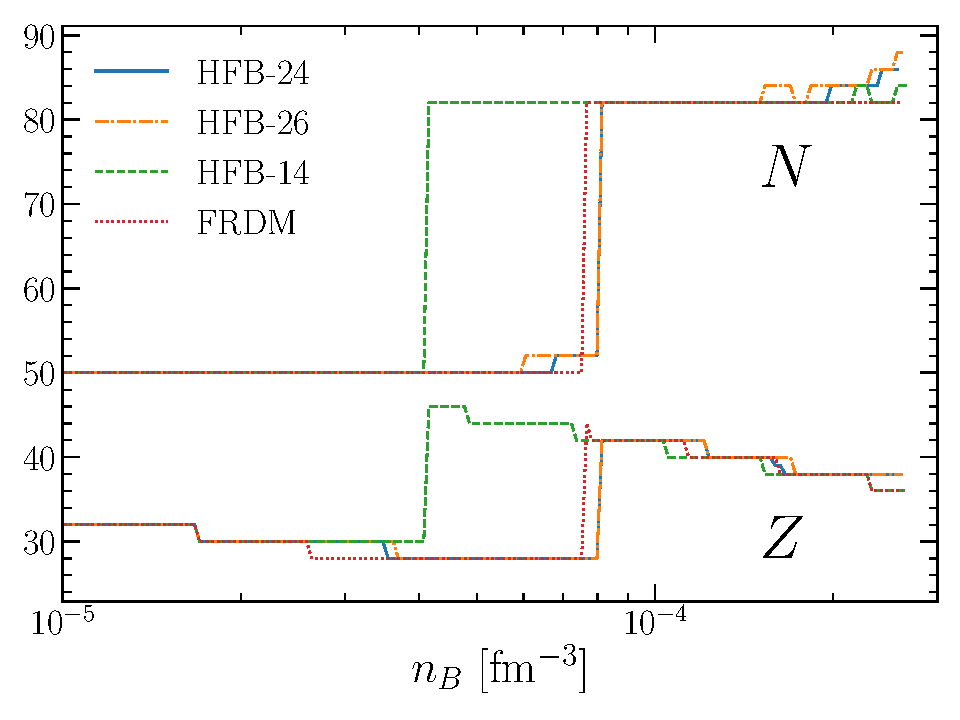
\includegraphics[width=0.8\linewidth]{figures/ocrust_model.pdf}
\end{center}
\caption[Ground-state composition versus baryon density in the 
outer crust]{Variation with baryon density $n_B$ of the equilibrium value of 
  atomic number $Z$ and neutron number $N$ in the bottom layers of the outer 
  crust for four different models: HFB-24, HFB-26~\cite{Goriely2013}, 
  HFB-14~\cite{Goriely2007}, and the FRDM~\cite{Moller1995}.}\label{fig:ocrust_model}
\end{figure}

The model dependence of the composition in the bottom layers of the outer crust 
(bottom part of Table~\ref{table:ocrust}) can be seen in
Figure~\ref{fig:ocrust_model}, where we represent the proton number $Z$ and the
neutron number $N$ as a function of the baryon density $n_B$ for four different
mass models that reproduce with comparable accuracy the present experimental
mass information: HFB-14~\cite{Goriely2007}, HFB-24, HFB-26~\cite{Goriely2013}, 
and the FRDM~\cite{Moller1995} that supplement the experimental data. The model
dependence is observed from $n_B \approx 2.5\times 10^{-5}$ fm$^{-3}$, where
the experimental mass data are not available. We 
recover similar sequences of nuclides with the different mass models, with
the strong shell effect associated to $N=50$ at low density and $N=82$ in the
bottom layers. A thin layer with $N=52$ is also found for HFB-24 and HFB-26 just before the
transition to $N=82$. While this transition occurs in the vicinity of $\approx 8\times
10^{-5}$ fm$^{-3}$ for HFB-24, HFB-26, and the FRDM, it is found to happen at
approximately $4\times 10^{-5}$ fm$^{-3}$ for HFB-14. Different nuclides are 
found close to the neutron drip, depending on the model: $^{124}$Sr is found for
HFB-24, $^{126}$Sr for HFB-26, $^{120}$Kr for HFB-14, and $^{122}$Kr for the FRDM. 
The neutron drip density $n_{ND}$ and pressure $P_{ND}$ slightly depends on 
the model as well. These values are reported in Table~\ref{table:drip}.

\begin{table}
\begin{center}
\begin{tabular}{cccccc} 
  \toprule
  \toprule
  model & element & $Z$ & $N$ & $n_{ND}$ (fm$^{-3}$) & $P_{ND}$ (MeV/fm$^3$)\\
  \midrule
  HFB-24 & $^{124}$Sr & 38 & 86 & $2.56\times 10^{-4}$ & $4.87\times 10^{-4}$\\
  HFB-26 & $^{126}$Sr & 38 & 88 & $2.62\times 10^{-4}$ & $4.91\times 10^{-4}$\\
  HFB-14 & $^{120}$Kr & 36 & 84 & $2.67\times 10^{-4}$ & $5.01\times 10^{-4}$\\
  FRDM   & $^{122}$Kr & 36 & 82 & $2.62\times 10^{-4}$ & $4.99\times 10^{-4}$\\
  \bottomrule
  \bottomrule
\end{tabular}
\end{center}
\caption[Ground state of matter at the neutron-drip point]{Chemical element, atomic 
  number $Z$, neutron number $N$, density
$n_{ND}$, and pressure $P_{ND}$ at the neutron drip point for four different
mass models: HFB-24, HFB-26~\cite{Goriely2013}, HFB-14~\cite{Goriely2007}, and
the FRDM~\cite{Moller1995}.}\label{table:drip} 
\end{table}

\begin{figure}[!t]
\begin{center}
  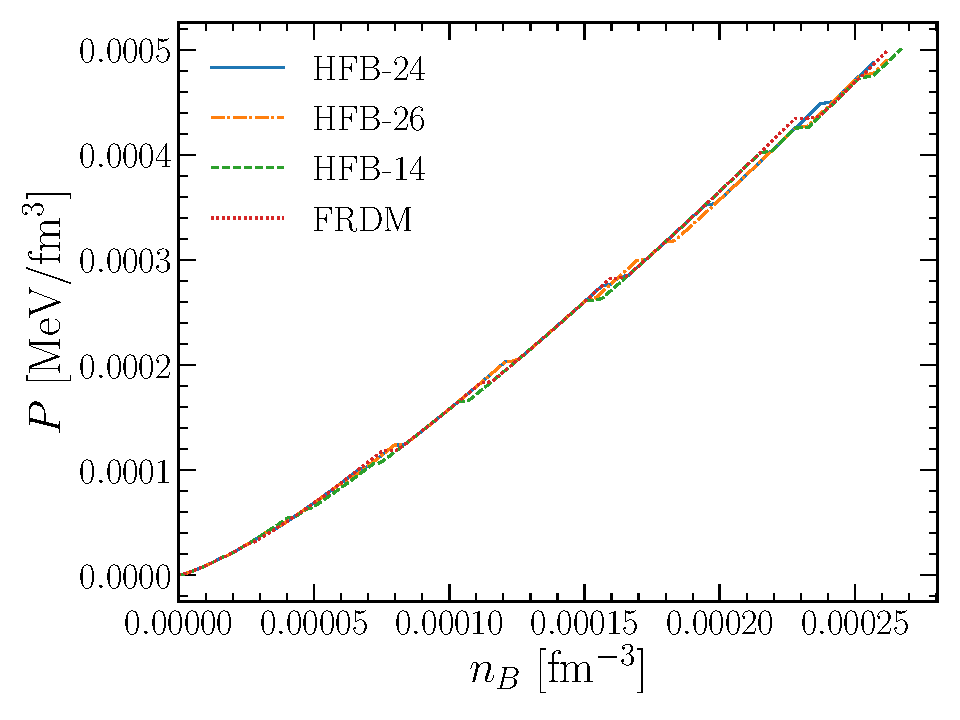
\includegraphics[width=0.8\linewidth]{figures/ocrust_pres.pdf}
\end{center}
\caption[Pressure versus baryon density in the outer crust]{Variation with 
  baryon density $n_B$ of pressure $P$ for four different models: HFB-24, 
  HFB-26~\cite{Goriely2013}, HFB-14~\cite{Goriely2007}, and the 
FRDM~\cite{Moller1995}.}\label{fig:ocrust_pres}
\end{figure}

The variation of pressure with baryon density, namely the EoS, is shown in
Fig.~\ref{fig:ocrust_pres} for the four mass models. The selected models give 
the same value of pressure up to $\approx 2.5\times10^{-5}$ fm$^{-3}$, as it is 
the case for the composition. At higher densities, we can perceive the small 
effect of the model, in particular at the transitions from a layer to another 
at which the pressure stays constant, but where a discontinuity is observed in 
the density.

% -----------------------------------------------------------------------------

\section{Ground state of the inner crust}\label{sec:icrust_gs}

The neutron drip marks the onset of the inner crust, which is a system that
cannot be reproduced in the laboratory since the dripped neutrons would
evaporate, while they stay confined in the WS cell due the gravitational
pressure. For this reason, the equilibrium composition and so the EoS in the 
inner crust are fully model dependent.

This section deals with the determination of the ground state of the inner
crust. In~\ref{subsec:nucenergy}, we present the metamodeling of the
infinite nuclear matter EoS here used to calculate the energy of the neutron 
gas, and extended to finite nuclei within the so-called compressible liquid 
drop (CLD) approximation so as to describe the cluster energetics. The derivation of the 
system of equilibrium equations for the determination of inner-crust ground state 
is detailed in~\ref{subsec:formalism}. The numerical
method as well as results are presented afterwards, 
in~\ref{subsec:results_icrust}. In~\ref{subsec:strutinsky} we add Strutinsky
shell corrections on top of the CLD energy as an attempt to recover magic
numbers in the free neutron regime. Nonspherical pasta phases in the bottom 
layers of the inner crust are considered in~\ref{subsec:pasta}. Finally, the
phase transition from the solid crust to the liquid core is investigated 
in~\ref{subsec:ccfromc}.

\subsection{Modeling the nuclear energy}\label{subsec:nucenergy}

% composition ws cell:
Once the neutron dripline is reached, neutron start to drip out of nuclei but
stay confined in the WS cell because of the gravitational pressure,
whereas they would have been emitted in the laboratory. In the regime of the inner
crust, we thus have, in each unit cell, a cluster immersed in an electron sea, 
and an ambient neutron gas.

\begin{figure}[!t]
\begin{center}
  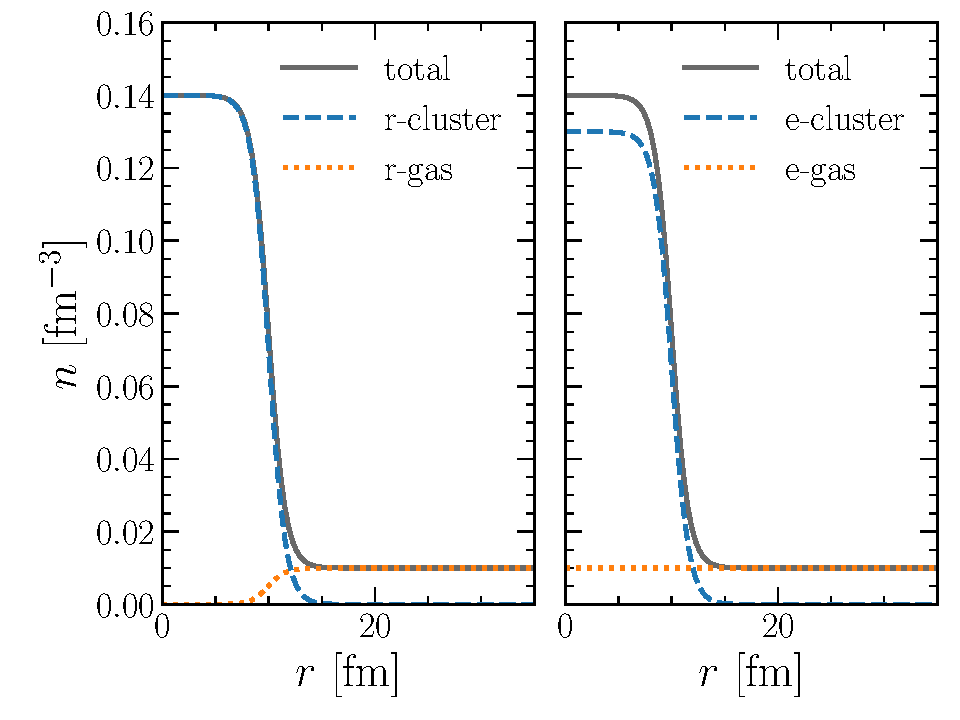
\includegraphics[width=0.9\linewidth]{figures/clustering.pdf}
\end{center}
\caption[\edit{r-cluster and e-cluster representations}]{\edit{Wood-Saxon 
    density profiles, for arbitrary values, within a WS cell in the free 
neutron regime. Blue dashed lines correspond to the cluster density (left,
r-cluster; right, e-cluster), and orange dotted lines to the gas density. The
total density profile is represented in gray solid lines.}}\label{fig:clustering}
\end{figure}

There is an ambiguity regarding the characterization of the cluster-gas
interface. One should ask whether the neutron gas penetrate the cluster or not.
Hence, two classical representations can be introduced, namely the r-cluster and
e-cluster representations~\cite{Papakonstantinou2013}, to interpret the
distribution
of the $N_{WS}$ neutrons and $Z_{WS}$ protons in the unit cell. In the former, the
cluster occupy a volume at the center of the cell and is surrounded
by the neutron gas. Evidently, there is a thin region where cluster and gas
overlap given the fact that a sharp interface would be unrealistic. The
r-cluster representation naturally emerges in the local density approximation
in density functional theory. Indeed, if the energy is expressed as a function
of the local density, then the cluster corresponds to the dense part and the
gas to the dilute one. This interpretation is used in most of the calculations
at finite temperature to model supernovae, see for example the renowned
Lattimer and Swesty EoS~\cite{Lattimer1991}. In the e-cluster representation,
the gas penetrate the cluster. This interpretation appears spontaneously in
single-particle developments. Indeed, in very neutron-rich clusters, beyond the
neutron dripline, the bound states are occupied as well as the resonant and
continuum states. All the unbound single-particle states that are occupied thus
represents the neutron gas, characterized by a quasihomogeneous spatial 
distribution, the continuum wave functions being very similar to plane waves.
\edit{The difference between the two representations is illustrated in 
Fig.~\ref{fig:clustering}. The cluster and gas density profiles, described by
Woods-Saxon profiles with arbitrary values, are plotted along the WS cell 
radius in the r-cluster representation (left) and e-cluster representation 
(right). Woods-Saxon profiles are known to give a good description of 
medium-mass and heavy nuclei density profiles, and are commonly used in
Thomas-Fermi (TF) and extended Thomas-Fermi (ETF) 
calculations \cite{Onsi2008,Pearson2018}. In both representations, the total
density profile (solid gray line) is the same.}\\
One can benefit from the advantage of both representations through the simple
geometric relations
%
\begin{equation}
  A_e = A\left(1-\frac{n_g}{n_0}\right), \quad 
  Z_e = A\left(1-\frac{n_{g,p}}{n_{0,p}}\right),
\end{equation}
%
where $A_e$ ($Z_e$) is the number of nucleons (protons) in the e-cluster, $A$
($Z$) the number of nucleons (protons) in the r-cluster, $n_g$ ($n_{g,p}$) the 
total (proton) gas density, and $n_0$ ($n_{0,p}$) the average total (proton) 
density inside the cluster. Since we do not consider the possibility of proton 
drip in the inner crust, we have $n_{g,p} = 0$, yielding $Z_e = Z$ and implying
that the total gas density is equal to that of the neutron gas. Indeed, 
while free protons are expected at non-zero temperature, their presence at zero 
temperature remains uncertain~\cite{BBP} and depends on the nuclear model. For 
some models, the proton drip could set in the very bottom layers of the crust, 
the classical condition for which is $\mu_p = U_p + m_pc^2$, where $U_p$ 
corresponds to the proton single-particle field at the cell 
surface~\cite{Pearson2018}. However, if nonspherical shapes are considered 
then it is found that protons remain in the cluster for most models.

At zero temperature, we write the WS cell energy $E_{WS}$ in the r-cluster 
representation as
%
\begin{equation}
  E_{WS} = E_{cl} + V_{WS}\varepsilon_e +
  (V_{WS}-V_{cl})\varepsilon_g + Z_{WS}(m_p - m_n)c^2 + A_{WS}m_nc^2\label{eq:ews_icrust}
\end{equation}
%
where $\varepsilon_g$ represents the energy density of the surrounding neutron gas
of density $n_g$, $V_{cl}=A/n_0$ the volume of the cluster, $V_{WS}$ that of
the WS cell, and $E_{cl}$ the energy of the cluster. The total number of
protons $Z_{WS}$ and nucleons $A_{WS}$ inside the WS cell are given respectively by
%
\begin{equation}
  Z_{WS} = A\frac{1-I}{2} \quad \text{and} \quad A_{WS} =
  A\left(1-\frac{n_g}{n_0}\right) + n_gV_{WS}.
\end{equation}
%
Let us notice that the number of protons inside the cell remains an
integer number, as in the outer crust, unlike the number of neutrons that is
noninteger because of the outside neutron gas.

As for the bottom layers of the outer crust, the determination of the ground 
state of the inner crust is fully model dependent.
Therefore, the two necessary ingredients of the WS cell energy are the 
equation of state of PNM, and the energy of the cluster, 
which will be treated in the CLD approximation 
introduced by Baym, Bethe, and Pethick (BBP) in their pioneering work~\cite{BBP}.

\subsubsection{Metamodeling of homogeneous nuclear matter}\label{subsubsec:hnm}

% description of infinite nuclear matter:
The ambient neutron gas in the WS cell is treated as homogeneous nuclear
matter.
In this limit, a large number of nucleons $A\longrightarrow \infty$ is 
contained in a large box. The system is entirely characterized by the neutron 
density $n_n$ and the proton density $n_p$. Let us also introduce the total 
density $n = n_n + n_p$ and the asymmetry $\delta = (n_n - n_p)/n$.
Two limit cases can be distinguished: pure neutron matter, where $n_p=0$,
and symmetric nuclear matter, where $n_n = n_p$. Beta-equilibrated 
matter corresponds to the matter inside the core of neutron stars and is 
treated in Section~\ref{sec:core}. Different methods have been proposed in
order to evaluate the energy per nucleon of homogeneous nuclear matter. While 
considerable theoretical efforts have been devoted to ab initio
approaches in the recent years~\cite{Gandolfi2014}, these calculations might 
become unreliable at suprasaturation densities. Also, the treatment of 
three-body forces, which are known to play a major role in the determination of 
the saturation properties of nuclear matter, remains a
challenge~\cite{Drischler2016}. Another possibility is to derive the nuclear 
EoS from effective forces~\cite{Chabanat1998}. This second approach is very 
practical because of translational invariance but suffers from the possible 
introduction of artificial correlations among the parameter space. In the 
following we present the metamodeling 
technique~\cite{Margueron2018a,Margueron2018b}. As we will see, this technique
allows to parametrize in a simple analytical way the energy per nucleon
obtained in the different ab initio or effective approaches, as well as
interpolate continuously between them. By largely exploring the parameter space
of this metamodel (or model of models), constraints coming from experimental
measurements can be directly implemented. Indeed, nuclear experiments give us 
knowledge on the properties of nuclear
matter around the saturation density of symmetric nuclear matter $n_{sat}$,
which is roughly the density of laboratory nuclei. For
instance, the isoscalar Giant Monopole Resonance energy is correlated
with the empirical parameter $K_{sat}$, which corresponds to the isoscalar
modulus.
%
\begin{table}
\begin{center}
\begin{tabular}{ccccccccc} 
  \toprule
  \toprule
  Parameter & Unit & $N$ & SLy4 & BSk24 & BSk22 & DD-ME$\delta$ & Average & Uncertainty\\
  \midrule
  $E_{sat}$ & MeV & 0         & -15.97 & -16.05  & -16.09    & -16.12 & -15.8 & 0.3   \\
  $n_{sat}$ & fm$^{-3}$ & 1   & 0.1595 &  0.1578 & 0.1578    & 0.1520 & 0.155 & 0.005 \\ 
  $K_{sat}$ & MeV & 2         & 230    &  246    & 246       & 219    & 230   & 20    \\ 
  $Q_{sat}$ & MeV & 3         & -363   &  -274.5 & -276      & -748   & 300   & 400   \\ 
  $Z_{sat}$ & MeV & 4         & 1587   &  1184   & 1190      & 3950   & -500  & 1000  \\ 
  $E_{sym}$ & MeV & 0         & 32.01  &  30.00  & 32.00     & 32.35  & 32    & 2     \\
  $L_{sym}$ & MeV & 1         & 46.0   &  46.4   & 68.5      & 52.8   & 60    & 15    \\
  $K_{sym}$ & MeV & 2         & -120   &  -38    & 13        & -118   & -100  & 100   \\
  $Q_{sym}$ & MeV & 3         & 521    &  711    & 563       & 846    & 0     & 400   \\
  $Z_{sym}$ & MeV & 4         & -3197  &  -4031  & -3174     & -3545  & -500  & 1000  \\
  $m_{sat}^*/m$ & &           & 0.69   &  0.80   & 0.80      & 0.69   & 0.75  & 0.1   \\
  $\Delta m_{sat}^*/m$ & &    & -0.19  &  0.20   & 0.20      & -0.17  & 0.1   & 0.1   \\
  \bottomrule
  \bottomrule
\end{tabular}
\end{center}
\caption[Empirical parameters for SLy4, BSk24, BSk22, and DD-ME$\delta$, and
extracted from nuclear experiments]{Value of each of the empirical parameters, 
  associated unit, and derivative order $N$ for 
  SLy4 \cite{Chabanat1998}, BSk24, BSk22~\cite{Goriely2013}, and 
  DD-ME$\delta$ \cite{RocaMaza2011} functionals.
Average values and uncertainties extracted from experimental analysis are taken
from \cite{Margueron2018a}.}\label{table:emp_params}
\end{table}
%
The well-known nuclear EoS empirical parameters correspond in fact to the 
successive density derivatives of nuclear matter energy per particle of SNM 
and symmetry energy at saturation density, associated to the isoscalar
($E_{sat}$, $K_{sat}$, $Q_{sat}$, and $Z_{sat}$) and isovector channel ($E_{sym}$,
$L_{sym}$, $K_{sym}$, $Q_{sym}$, and $Z_{sym}$), respectively. 
The symmetry energy is generally defined as
%
\begin{equation}
  e_{HM}^{sym}(n) = \frac{1}{2}\frac{\partial^2 e_{HM}(n,\delta)}{\partial
  \delta^2}\bigg|_{\delta=0},\label{eq:esym}
\end{equation}
%
where $e_{HM}$ is the nuclear matter energy per nucleon in nuclear matter. In
Table~\ref{table:emp_params} are listed the value of each empirical parameter
for the Skyrme-like SLy4~\cite{Chabanat1998}, BSk22, and
BSk24~\cite{Goriely2013}, and relativistic
DD-ME$\delta$~\cite{RocaMaza2011} functionals. Average values and associated
uncertainties extracted from experimental analysis are also provided. It can be
seen that the isovector parameters are in general less known with respect to
the isoscalar ones for the same derivative order. For instance, the relative
uncertainty on $K_{sym}$ is about $100\%$ while that of $K_{sat}$ is less than
$10\%$. It should also be stressed that high-order parameters $Q_{sat(sym)}$
and $Z_{sat(sym)}$ are poorly constrained by nuclear experiments.\\
The empirical parameters can be used in a Taylor expansion to estimate the
nuclear matter EoS analytically up to 
$n \approx 2-3n_{sat}$~\cite{Margueron2018a,Margueron2018b}. Limiting us to 
derivative order $N=2$, we obtain
%
\begin{equation}
  e^{N=2}_{HM}(n,\delta) = E_{sat} + \frac{1}{2}K_{sat}x^2 
  + \delta^2 (E_{sym} + L_{sym}x +\frac{1}{2}K_{sym}x^2),
\end{equation}
%
with $x = (n-n_{sat})/(3n_{sat})$ a function of the density. \edit{However, we 
  should stress already that $N=2$ is not sufficient for describing the EoS at 
  subsaturation densities, and even less for suprasaturation densities. 
  High-order parameters $Q_{sat(sym)}$ and $Z_{sat(sym)}$ are essential and 
  carry the largest uncertainty as far as the bulk part of the EoS is 
concerned.}

In a mean field approach, we can treat nucleons as independent
particles, thus the kinetic part of the energy per particle of nuclear matter 
is given by the same functional form as a nonrelativistic Fermi gas (FG), that 
is
%
\begin{equation}
  t_{HM}^{FG}(n,\delta) =
  \frac{1}{2}t_{sat}^{FG}(1+3x)^{2/3}\left[(1+\delta)^{5/3}\frac{m}{m_n^*} +
  (1-\delta)^{5/3}\frac{m}{m_p^*}\right],
\end{equation}
%
where $t_{sat}^{FG} = 3\hbar^2/(10m)(3\pi^2/2)^{2/3}n_{sat}^{2/3}$ is the
kinetic energy of SNM at the saturation density, $m = (m_n + m_p)/2$ is the
mean nucleon mass, and $m_n^*$ ($m_p^*$) is the neutron (proton) effective
mass. The Landau effective mass is introduced in order to take into account for 
the in-medium nuclear interaction that alters the mass of nucleons. It can be
parametrized as ($q=n,p$)
%
\begin{equation}
  \frac{m}{m_q^*} = \sum_{\alpha=0}^1
  m_{q,\alpha}(\delta)\frac{x^\alpha}{\alpha!}
  = 1 + (\kappa_{sat} + \tau_3\kappa_{sym}\delta)(1+3x),
\end{equation}
%
with $\tau_3 = 1$ ($\tau_3 = -1$) for neutrons (protons).
Two additional parameters $\kappa_{sat}$ and $\kappa_{sym}$, related to the 
effective mass $m_{sat}^*$ and isospin splitting $\Delta m_{sat}^*$ at 
saturation density, are then introduced. They are defined at $n = n_{sat}$ as
%
\begin{eqnarray}
  \kappa_{sat} &=& \frac{m}{m_{sat}^*} - 1,\\
  \kappa_{sym} &=& \frac{1}{2}\left(\frac{m}{m_n^*} - \frac{m}{m_p^*}\right).
\end{eqnarray}
%

\edit{In principle, it is possible to reproduce any EoS model with a Taylor
  expansion, considering an infinite number of parameters,
  $N\rightarrow\infty$, however the convergence would be very slow. In order to 
  fasten the series convergence, one can add extra functional dependencies, 
  which correspond to the true EoS in the limit of simplistic cases 
  (independent particles, zero density limit), but which allow, by judicious
  choices of empirical parameters, to reproduce with precision realistic 
functionals.}
\edit{In this regard}, the $\delta^{5/3}$ dependence is added by decomposing 
the energy per particle into a potential and kinetic part, yielding
%
\begin{equation}
  e^N_{HM}(x,\delta) = t_{HM}^{FG}(n,\delta) +
  v_{MM}^N(n,\delta),\label{eq:meta}
\end{equation}
%
where $v_{MM}^N$ is the potential energy per particle expressed as a Taylor expansion
in the parameter $x$ at $n = n_{sat}$,
%
\begin{equation}
  v_{MM}^N(n,\delta) = \sum_{\alpha \geq 0}^N(v_\alpha^{is} +
  \delta^2v_\alpha^{iv})\frac{x^\alpha}{\alpha!}\label{eq:elfa}.
\end{equation}
%
The quadratic approximation for the isospin dependence of the potential energy 
has been made in Eq.~(\ref{eq:elfa}), as suggested by microscopic calculations 
in~\cite{Vidana2009}. The coefficients $v_\alpha^{is}$ and $v_\alpha^{iv}$ are
mapped to the empirical parameters following
%
\begin{equation}
  v_\alpha^{is} = \frac{\partial^\alpha e_{HM}}{\partial
  x^\alpha}\bigg|_{n=n_{sat},\delta=0} \quad \text{and} \quad v_\alpha^{iv} = \frac{\partial^\alpha e_{HM}^{sym}}{\partial
x^\alpha}\bigg|_{n=n_{sat},\delta=0},\label{eq:def_pars}
\end{equation}
%
yielding the isoscalar parameters:
%
\begin{eqnarray}
  v_0^{is} &=& E_{sat} - t_{sat}^{FG}(1+\kappa_{sat}),\\
  v_1^{is} &=& -t_{sat}^{FG}(2+5\kappa_{sat}),\\
  v_2^{is} &=& K_{sat} - 2t_{sat}^{FG}(-1+5\kappa_{sat}),\\
  v_3^{is} &=& Q_{sat} - 2t_{sat}^{FG}(4-5\kappa_{sat}),\\
  v_4^{is} &=& Z_{sat} - 8t_{sat}^{FG}(-7+5\kappa_{sat}),
\end{eqnarray}
%
and isovector parameters:
%
\begin{eqnarray}
  v_0^{iv} &=& E_{sym} - \frac{5}{9}t_{sat}^{FG}[1+(\kappa_{sat}+3\kappa_{sym})],\\
  v_1^{iv} &=& L_{sym} - \frac{5}{9}t_{sat}^{FG}[2+5(\kappa_{sat}+3\kappa_{sym})],\\
  v_2^{iv} &=& K_{sym} - \frac{10}{9}t_{sat}^{FG}[-1+5(\kappa_{sat}
  +3\kappa_{sym})],\\
  v_3^{iv} &=& Q_{sym} - \frac{10}{9}t_{sat}^{FG}[4-5(\kappa_{sat}+3\kappa_{sym})],\\
  v_4^{iv} &=& Z_{sym} -
  \frac{40}{9}t_{sat}^{FG}[-7+5(\kappa_{sat}+3\kappa_{sym})],
\end{eqnarray}
%

Let us notice from Eq.~(\ref{eq:elfa}) that the energy per particle does not 
converge to zero at zero density. This artifact, arising from the nature of the 
series expansion, can be fixed by introducing an exponential correction 
$u^N_\alpha(x)$ in the potential energy, 
%
\begin{equation}
  v_{MM}^N(n,\delta) = \sum_{\alpha \geq 0}^N(v_\alpha^{is} +
  \delta^2v_\alpha^{iv})\frac{x^\alpha}{\alpha!}u_\alpha^N(x),\label{eq:mm}
\end{equation}
% 
the expression of which is
%
\begin{equation}
  u_\alpha^N(x) = 1 - (-3x)^{N+1-\alpha}\exp(-b(1+3x)),\label{eq:corr}
\end{equation}
%
where we have introduced an extra low-density parameter $b$. It was shown in
\cite{Antic2019} that for most applications this parameter can be fixed to a
constant, $b=10\ln(2)$.

Let us now turn to the derivatives of the energy. The expression of the 
symmetry energy, Eq.~(\ref{eq:esym}), reads
%
\begin{equation}
  e_{HM}^{sym}(n) =
  \frac{5}{9}t_{sat}^{FG}(1+3x)^{2/3}
  \left[1+(\kappa_{sat}+3\kappa_{sym})(1+3x)\right] + \sum_{\alpha \geq 0}^N
  v_{\alpha}^{iv}\frac{x^{\alpha}}{\alpha!}u_{\alpha}^N(x).\label{eq:esym_exp}
\end{equation}
%
For the chemical potential, we have
%
\begin{equation}
  \mu_{HM,q}(n,\delta) = e_{HM}^N 
  + \frac{1+3x}{3}\left(\frac{\partial e_{HM}^N}{\partial x}\right)_{\delta}
  + (\tau_3 - \delta)\left(\frac{\partial e_{HM}^N}{\partial \delta}\right)_{x} 
  + m_{q} c^2,\label{eq:chempot}
\end{equation}
%
The complete analytical expression of $\mu_{HM,q}$ is given in Appendix 
\ref{appendix:mutau}. Finally, the pressure can be calculated through
%
\begin{equation}
  P_{HM} = \sum_{q=n,p}n_{q}(\mu_{HM,q}(n,\delta) - m_{q}c^2) 
  - ne_{HM}^N(n,\delta).\label{eq:phm}
\end{equation}
%

There are two main advantages that come with the metamodeling technique.\\
Firstly, It is flexible enough to reproduce the different existing energy functional of 
nuclear matter with very good accuracy up to $n \approx 2-3n_{sat}$, and even higher
densities with a proper redefinition of the third and fourth order 
parameters~\cite{Margueron2018a}. Since very often the
parameters of the model to be mimicked do not coincide with the empirical
parameters, we derive the latter by calculating the derivatives of the energy 
per particle in nuclear matter at saturation density, following
Eq.~(\ref{eq:def_pars}).
%
\begin{figure}[!t]
\begin{center}
  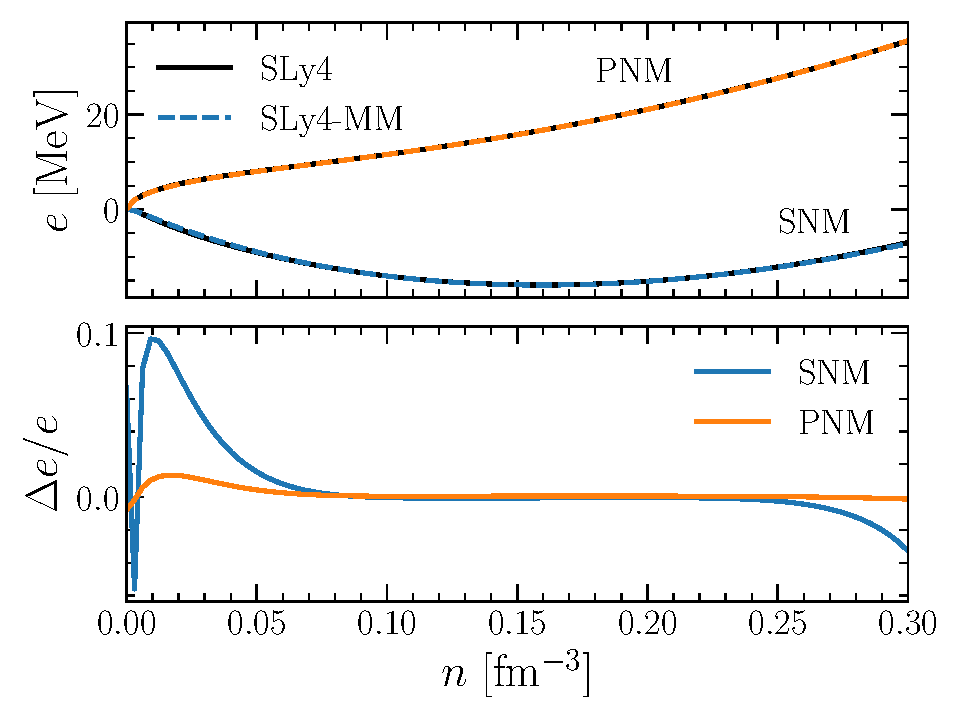
\includegraphics[width=0.9\linewidth]{figures/mm_accuracy.pdf}
\end{center}
\caption[Accuracy of the metamodeling technique for SLy4]{Energy per 
  nucleon as a function of density for symmetric
  nuclear matter, $\delta=0$, and pure neutron matter, $\delta=1$ (upper panel), and the
associated relative error $\Delta e/e = (e_{MM} - e)/e$ (lower panel) for the SLy4
functional, with $N=4$ for the metamodel. In the top panel, black solid lines 
(dashed lines) correspond to the
calculation with the exact functional (metamodel).}\label{fig:mm_accuracy}
\end{figure}
%
In Fig.~\ref{fig:mm_accuracy} is demonstrated the accuracy of the metamodeling
technique for the SLy4~\cite{Chabanat1998} functional with a Taylor expansion 
order $N=4$. In the top panel, the energy per nucleon is calculated 
using the metamodeling technique (dashed lines) and the exact functional (black
solid lines). A tiny deviation is observed at low density for the SNM, but 
overall a very good agreement is observed between the metamodel (labeled
``SLy4-MM'') and the exact functional (labeled ``SLy4''). In the lower panel 
the relative error is represented for
SNM and PNM. We can see that the error goes up to $10\%$ for SNM at $n \approx
0.01$ fm$^{-3}$ and rapidly drops to $0\%$ at $n \approx 0.07$
fm$^{-3}$. At $n \approx 2n_{sat}$, a deviation appears due the extrapolation far
from the saturation point. The deviation at low density can be reduced by 
adjusting the parameter $b$ entering in the low-density correction,
Eq.~(\ref{eq:corr}) \cite{Antic2019}. However,
this small deviation is not expected to cause any issue for the determination
of the inner crust ground state. Indeed, the relative error for PNM is lower 
that $2\%$ at most, and, in the inner crust, the matter inside nuclei is very 
neutron rich and the ambient nucleon gas is exclusively constituted of free
neutrons. \edit{This ability of mimicking existing realistic functionals will 
  allow us to easily compare predictions of astrophysical observables of 
different popular models.}\\
Another asset of the metamodeling technique is that no correlation is assumed
a priori among the empirical parameters due to the nature of the
series expansion. Therefore, all density dependences of the
nuclear EoS can be explored. In addition, it allows us to vary each empirical 
parameter independently of the others to carry out complete statistical 
analysis using Bayesian inference. 
% In that sense, a sensitivity study on
% the nuclear EoS in performed in~\cite{Margueron2018a} in order to observe which
% parameters are the most influential. The conclusion was that the lowest order
% empirical parameters which require to be better constrained -- either from
% nuclear experiments or astrophysical observations -- are $Q_{sat}$ in 
% the isoscalar channel, and $L_{sym}$ and $K_{sym}$ in the isovector one.

\subsubsection{From homogeneous nuclear matter to finite nuclei in the CLD 
approximation}\label{subsubsec:cld}

% need to expand the model to account for the finite surface of nuclei:
We now turn to the modeling of the energy of clusters present in the inner crust
of cold neutron stars. We propose to extend the metamodeling of infinite nuclear 
matter to nuclei in order to take into account their surface properties, within 
the CLD approximation, originally
introduced in~\cite{BBP}. This approach is 
expected to be less accurate than microscopic Hartree-Fock
(HF)~\cite{Negele1973} or (ETF)~\cite{Onsi2008} 
calculations since quantum effects are neglected, 
though it proved its quality in the past by giving surprisingly good
results, see for example~\cite{BBP,Lattimer1991,Douchin2000a,Douchin2001}. 
In particular, it
appears that most of the macroscopic observables related to neutron stars, such 
as masses and radii, are not very sensitive to the crust composition, thus a 
qualitative evaluation of it is sufficient in that case.
% advantages and disadvantages:
The compressible liquid drop model (CLDM) comes with multiple advantages. It is
very fast from the computational point of view since the energy does not require
to be integrated all along the cell volume.
For this reason, it is powerful for complete statistical analyses such as the one 
presented in the next chapter. It is also a model that is \edit{flexible}, giving 
us the opportunity to account for different geometries for example, as we 
consider in \ref{subsec:pasta}. Last but not 
least, because of the artificial decomposition of the nuclear cluster as a 
bulk term, a surface term, and a Coulomb term, we are able to identify the
contributions of the different terms. For all these reasons, the CLDM is
considered as a suitable alternative to semiclassical ETF and microscopic 
HF treatments, that additionally does not suffer from technical
complications such as the definition of boundary conditions~\cite{Newton2009}.

In the CLD approximation, the energy of the cluster reads
%
\begin{equation}
  E_{cl} = e_{HM}(n_0, I)A + E_{surf} + E_{Coul},
\end{equation}
%
where $E_{surf}$ represents the nuclear surface energy, and $E_{Coul}$ is the Coulomb
energy, including the lattice correction and finite-size effects, written 
as follows in the WS approximation,
%
\begin{equation}
  E_{Coul} = \frac{3}{5}\frac{e^2}{r_0^2}\eta_{Coul}(u)\frac{Z^2}{A^{1/3}} =
  \frac{3}{20}\frac{e^2}{r_0^2}\eta_{Coul}(u)A^{5/3}(1-I)^2,\label{eq:ecoul}
\end{equation}
%
with
%
\begin{equation}
  \eta_{Coul}(u) = 1-\frac{3}{2}u^{1/3} + \frac{1}{2}u,\label{eq:fcoul}
\end{equation}
%
a function of the volume fraction $u = n_e/n_{0,p}$, with $n_{0,p} =
n_0(1-I)/2$ the average proton density inside cluster. Let us notice that, 
the factor $3/5 \times 3/2 = 9/10$ entering in the lattice term can be
replaced by the Mandelung constant for a body-centered cubic lattice, $C_M =
0.895929255682$ (see Table 2.4 of~\cite{Haensel2007}).\\
The bulk term is taken from the metamodel, keeping the same empirical parameters
as for the calculation of the neutron gas energy, thus insuring consistency
between the crust and the core treatment. 
The bulk energy is evaluated at $n_0$, the average density inside the cluster, 
and $I$, its global asymmetry.

Let us now turn to the expression of the nuclear surface energy. Assuming that
clusters are spherical, it is given by
%
\begin{equation}
  E_{surf} = 4\pi r_0^2A^{2/3}\sigma,\label{eq:esurf}
\end{equation}
%
where $r_0 = (4\pi n_0/3)^{-1/3}$ is related to the cluster density $n_0$, and
$\sigma$ is the nuclear surface tension. The simplest parametrization of the
surface tension one could use is a constant, $\sigma \approx 1.03$ MeV/fm$^2$, 
as in the liquid drop model. %ref ldm?
However, clusters in the inner crust are expected to be very neutron rich and
it appears evident that the surface tension of very asymmetric nuclei should be
different to that of symmetric nuclei. In addition, it does not account for
the interaction of the nuclear surface with the outside neutron gas, yielding 
$\sigma \rightarrow 0$ as $I\rightarrow 1$. 
This leads us to consider another parametrization for $\sigma$ which would 
depend on the asymmetry $I$ and consider the interaction with the gas.
It should be mentioned that the exact value of $\sigma(I)$ is model dependent, 
and the uncertainty is particularly important for extreme isospin values 
encountered in the inner crust. Indeed, no experimental data exist on the 
surface energy of nuclei beyond the dripline, which is in-medium modified by 
the presence of the neutron gas~\cite{Douchin2000b}.
We use the expression originally proposed by Ravenhall \textit{et
al.}~\cite{Ravenhall1983} on the basis of TF calculations at
extreme isospin ratios, and later employed in different works on neutron star
crust and supernovae modeling within the 
CLD approximation~\cite{Lattimer1991,Newton2012,Lorenz1993}:
%
\begin{equation}
  \sigma(I) = \sigma_0\frac{2^{p+1} + b_s}{Y_p^{-p} + b_s + (1 -
  Y_p)^{-p}},\label{eq:sigma}
\end{equation}
%
with $\bm{S} = \{\sigma_0, b_s, p\}$ the parameter space associated to the
surface energy. The parameter $\sigma_0 = \sigma(I=0)$ represents the surface 
tension of symmetric nuclei, and $b_s$ and $p$ are the parameters that govern 
the isospin dependence of the surface tension. The proton fraction is 
related to the asymmetry inside the cluster via $Y_p = (1-I)/2$. 
% curvature term:
Following~\cite{Newton2012}, we add a curvature term with the aim of having a
better description of the nuclear surface and so of the composition of the
inner crust in the ground state. For spherical clusters, the curvature energy
reads
%
\begin{equation}
  E_{curv} = 8\pi r_0A^{1/3}\sigma_c,\label{eq:ecurv}
\end{equation}
%
where $\sigma_c$ is the curvature tension related to the surface tension
$\sigma$, Eq.~(\ref{eq:sigma}),
%
\begin{equation}
  \sigma_c =
  \sigma\frac{\sigma_{0,c}}{\sigma_0}\alpha(\beta-Y_p),\label{eq:sigmac}
\end{equation}
%
with $\alpha = 5.5$ as in~\cite{Newton2012}. With the addition of the
curvature energy comes two parameters added as extra dimensions to 
the surface parameter space, $\bm{S} = \{\sigma_0, b_s, \sigma_{0,c}, \beta,
p\}$.
%
\begin{figure}[!t]
\begin{center}
  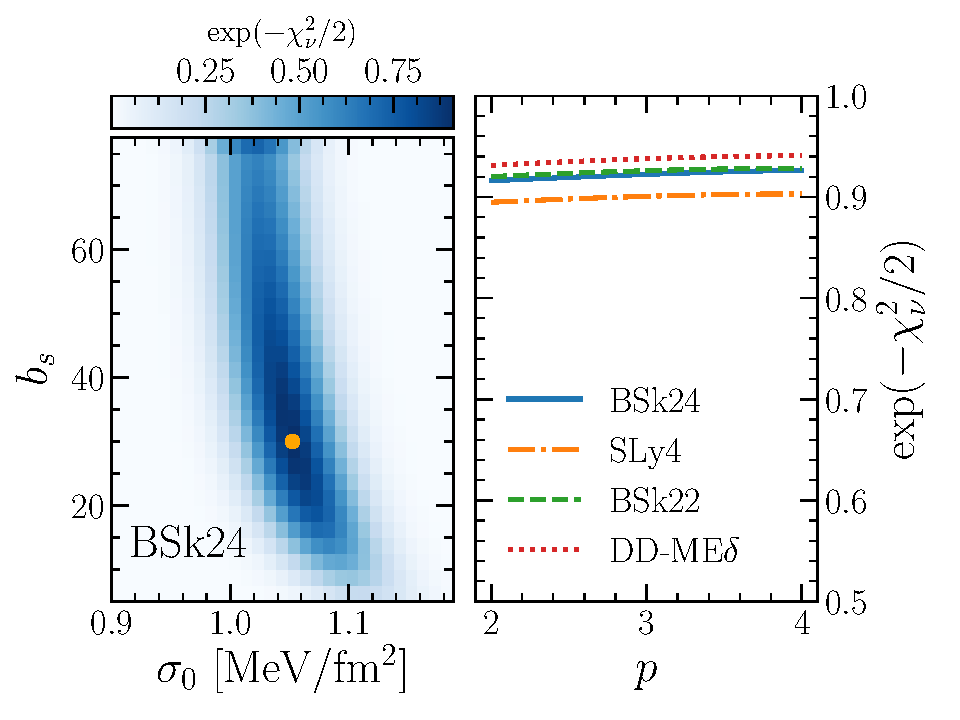
\includegraphics[width=0.9\linewidth]{figures/surf_fit.pdf}
\end{center}
\caption[\edit{Fit of surface and curvature parameters}]{\edit{Left: Goodness 
    of fit (color scale) as described 
    by the reduced $\chi^2$, in the space of the surface parameters 
    $(\sigma_0,b_s)$ for the BSk24 CLDM with fixed value of the $p$ parameter, 
$p=3$, for optimized curvature parameters $\sigma_{0c}$ and $\beta$. The orange 
point indicates the optimal value. Right: Weight $\exp(-\chi^2_\nu/2)$ as a 
function of the parameter $p$, calculated for the optimal value of
$(\sigma_0,b_s,\sigma_{0c},\beta)$, for the selected 
CLDM: BSk24, SLy4, BSk22, and DD-ME$\delta$.}}\label{fig:surf_fit}
\end{figure}
%
For a given model of uniform matter, that is each given set of empirical
parameters, the first four parameters can be fitted to experimental masses from 
the AME2016~\cite{Huang2017} for a fixed value of the parameter $p$. \edit{The
  quality of reproduction of the experimental nuclear binding energy
  $E_{\text{AME2016}}$ is measured by the reduced $\chi^2$, defined as
  %
  \begin{equation}
    \chi^2_\nu = \frac{\chi^2}{\nu} = \frac{1}{\nu}
    \sum_i\left(\frac{E_{cl}^{(i)}/A^{(i)}-E_{\text{AME2016}}^{(i)}/A^{(i)}}
    {\sigma^{(i)}}\right)^2,\label{eq:chi2}
  \end{equation}
  %
  where $\nu$ is the number of degrees of freedom, and the denominator
  corresponds to the systematic theoretical error, 0.1 MeV/$A$, such as to have
  $\chi^2_{min} \approx 1$ over the parameter space 
  sample \cite{Dobaczewski2014}.\\
  This point can be clearly understood by inspection of the left panel of
Fig.~\ref{fig:surf_fit}, which shows the value of the weight function 
$\exp(-\chi^2_\nu/2)$, that is the goodness of fit, in the 
$(\sigma_0,b_s)$ plane, for the BSk24 CLDM with 
$p=3$, and curvature parameters already adjusted to experimental data. It is
seen that the weight function is strongly peaked to the orange point, which
indicates the optimal value for the parameters $\sigma_0$ and $b_s$.
Conversely, we observe in the right panel of Fig.~\ref{fig:surf_fit} that the 
error estimator $\chi^2_\nu$ is insensitive to the choice of the parameter $p$ 
in a range going from 2 to 4, for four representative functionals. This is
understood from the fact that $p$ modifies the asymmetry dependence of the
surface energy only for extreme values of $I$ where nuclear data are not
available.} This parameter 
is \edit{therefore} not adjusted as the other parameters, in order to avoid 
poor extrapolations of $\sigma$. The value of $p$ is selected around $p=3$, 
which is the value used in the popular Lattimer and Swesty EoS~\cite{Lattimer1991}.
%
\begin{figure}[!t]
\begin{center}
  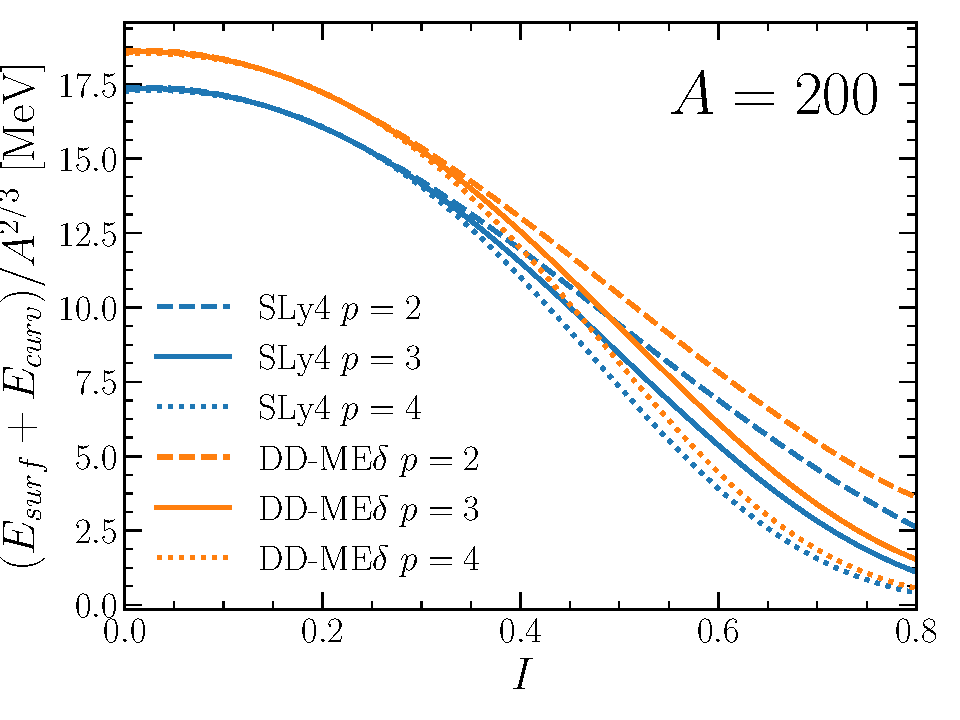
\includegraphics[width=0.8\linewidth]{figures/surfenpersurfnuc.pdf}
\end{center}
\caption[Surface plus curvature energy per surface nucleon versus asymmetry]{Variation 
  with cluster asymmetry $I$ of surface plus curvature energy per
  surface nucleon along the isobaric chain $A=200$ for SLy4~\cite{Chabanat1998} and
DD-ME$\delta$~\cite{RocaMaza2011} CLDM at three selected 
values of parameter $p$: $p=2$ (dashed lines), $p=3$ (solid lines), and $p=4$
(dotted lines).}\label{fig:surfenpersurfnuc}
\end{figure}
%
We show in Fig.~\ref{fig:surfenpersurfnuc} the surface plus curvature energy
per surface nucleon as a function of the asymmetry inside the cluster for two
popular models, SLy4~\cite{Chabanat1998} and DD-ME$\delta$~\cite{RocaMaza2011},
in the CLD approximation. Different values for the parameter $p$ are displayed 
in that figure. It is seen that $p$ determines the behavior of the surface
tension for extreme isospin values, and cannot be accessed from experimental
nuclear physics data. \edit{In addition, since the selected popular models contain
parameters that are adjusted to the same data, we cannot cannot consider their
predictions at high isospin as reliable. For these reasons, we will keep $p$ as 
a free parameter.} In particular, from $I \approx 0.3$, we observe that a 
larger value of $p$ leads to larger surface energy at fixed asymmetry. The
model dependence of the surface tension is also observed in that figure and is
particularly highlighted at low asymmetry where experimental measurements can 
still be performed.

Finally, we recall the final expression for the cluster binding energy in the
CLD approximation,
%
\begin{eqnarray}
  E_{cl}(A,I,n_0,n_e) =&& e_{HM}(n_0, I)A \notag \\
          &&+ 4\pi r_0^2A^{2/3}\sigma(I) + 8\pi r_0A^{1/3}\sigma_c(I) \notag \\
          &&+ \frac{3}{20}\frac{e^2}{{r_0}^2}\eta_{Coul}(I,n_0,n_e)A^{5/3}(1-I)^2.
          \label{eq:enuc}
\end{eqnarray}
%
Let us notice that the energy does not depend on the neutron gas density via
the surface term, as in~\cite{BBP}. This dependence is in fact implicitly
accounted for in the chosen parametrization of the surface tension, suggested 
from microscopic calculations in the WS cell~\cite{Ravenhall1983}.

\subsection{Variational formalism}\label{subsec:formalism}

The variational method for the calculation of the inner crust ground state
with the CLDM was introduced in the pioneering work of BBP 
in their classical paper~\cite{BBP}. Since then, huge progress has been
made in constraining the nucleon-nucleon (NN) effective interaction. For this 
reason, subsequent works using the same formalism with CLDM based on more 
realistic nuclear functionals followed. For instance we can mention the popular 
calculations of Douchin and Haensel (DH)~\cite{Douchin2000a, Douchin2000b} with 
the SLy4 effective force~\cite{Chabanat1998}. Following those works, we use the 
same variational method as BBP, and we present it in the following.

Using the Lagrange multipliers method, the ground state of the inner crust is
obtained by minimizing the zero-temperature free
energy density of the WS cell at fixed baryon density $n_B$ under the condition 
of charge neutrality, $n_e = n_p$. The minimization is carried out with 
respect to the set of variables $A$, $I$, $n_0$, $n_p$, and $n_g$.
Let us notice that, in principle, one should minimize the Gibbs free energy at 
constant pressure, as for the outer crust. However, it would be very heavy from 
the computational point of view to do so in the free neutron regime.
Fortunately, it is demonstrated that the error introduced by minimizing at
constant baryon density instead of pressure is negligible~\cite{Pearson2012}.
The auxiliary function to be minimized is defined as
%
\begin{eqnarray}
  \mathcal{L}(A,I,n_0,n_p,n_g) &=& \frac{E_{WS}}{V_{WS}} - \mu n_B \notag \\
                      &=& \frac{E_{cl}}{V_{WS}} + \varepsilon_e +
              \left(1-\frac{A}{n_0V_{WS}}\right)\varepsilon_g \notag\\
                      &&+ n_p \Delta m_{pn}c^2 - n_B(\mu -
                      m_nc^2),\label{eq:aux}
\end{eqnarray}
%
with $\Delta m_{pn} = m_p - m_n$ the difference between the proton and neutron
mass, and $\mu$ the Lagrange multiplier.\\
The volume of the cell can be calculated as
%
\begin{equation}
  V_{WS} = \frac{Z}{n_p} = \frac{A}{n_p}\frac{1-I}{2},
\end{equation}
%
and the baryon density is given by 
%
\begin{eqnarray}
  n_B &=& \frac{A_{WS}}{V_{WS}} \notag\\
      &=& \frac{2n_p}{1-I}\left(1-\frac{n_g}{n_0}\right) + n_g.
\end{eqnarray}
%
Replacing these quantities in Eq.~(\ref{eq:aux}), it results
%
\begin{eqnarray}
  \mathcal{L}(A,I,n_0,n_p,n_g) &=& \frac{2n_p}{A(1-I)}E_{cl} + \varepsilon_e +
  \left(1-\frac{2n_p}{n_0(1-I)}\right)\varepsilon_g 
                      + n_p \Delta m_{pn}c^2 \notag\\
                      &&- \frac{2n_p}{1-I}\left(1-\frac{n_g}{n_0}\right)(\mu - m_nc^2)
                      - n_g(\mu - m_nc^2).\label{eq:aux_final}
\end{eqnarray}
%

% min wrt A
Let us first minimize with respect to $A$:
%
\begin{eqnarray}
  \frac{\partial \mathcal{L}}{\partial A}\bigg|_{I,n_0,n_p,n_g} &=& 0 \notag\\
  \frac{2n_p}{A(1-I)}\frac{\partial E_{cl}}{\partial A} -
  \frac{2n_p}{A^2(1-I)}E_{cl} &=& 0 \notag\\
  \frac{\partial E_{cl}}{\partial A} - \frac{E_{cl}}{A} &=& 0,
\end{eqnarray}
%
which is equivalent to
%
\begin{equation}
  \frac{\partial (E_{cl}/A)}{\partial A} = 0.
\end{equation}
%
We can go trough this equation using the definition of the cluster energy, 
Eq.~(\ref{eq:enuc}), yielding
%
\begin{eqnarray}
  -\frac{1}{3}\times 4\pi r_0^2 \sigma A^{-4/3} - \frac{2}{3}\times 8\pi r_0\sigma_cA^{-5/3}
  + \frac{2}{3}\times\frac{3}{20}\frac{e^2}{r_0}\eta_{Coul}A^{-1/3}(1-I)^2 &=&
  0 \notag\\
  4\pi r_0^2 \sigma A^{2/3} + 2\times 8\pi r_0\sigma_cA^{1/3}
  - 2\times \frac{3}{20}\frac{e^2}{r_0}\eta_{Coul}A^{5/3}(1-I)^2 &=& 0 \notag,
\end{eqnarray}
or simply,
%
\begin{equation}
  E_{surf} + 2E_{curv} = 2E_{Coul}.\label{eq:virial}
\end{equation}
%
This equation corresponds to the well-known Baym virial theorem with an 
additional curvature term with respect to the equation originally found 
in~\cite{BBP}. It is interesting to notice that only the surface, the 
curvature, and the Coulomb energy are involved in this first equilibrium 
condition.

% min wrt ng
Minimizing with respect to the neutron gas density $n_g$, one obtains:
%
\begin{eqnarray}
  \frac{\partial \mathcal{L}}{\partial n_g}\bigg|_{A,I,n_0,n_p} &=& 0 \notag\\
  \left(1-\frac{2n_p}{n_0(1-I)}\right)\frac{\partial \varepsilon_g}{\partial
n_g} + \frac{2n_p}{n_0(1-I)}(\mu - m_nc^2) - (\mu - m_nc^2) &=& 0,
\end{eqnarray}
%
giving us the expression of the Lagrange multiplier, which can be identified
with the chemical potential of the gas, including the rest mass energy,
%
\begin{equation}
  \mu = \frac{\partial \varepsilon_g}{\partial n_g} + m_nc^2 \equiv
  \mu_g.\label{eq:lagrange}
\end{equation}
%

% min wrt n0
We now turn to the minimization with respect to average cluster density $n_0$:
%
\begin{eqnarray}
  \frac{\partial \mathcal{L}}{\partial n_0}\bigg|_{A,I,n_p,n_g} &=& 0 \notag\\
  \frac{2n_p}{A(1-I)}\frac{\partial E_{cl}}{\partial n_0} +
  \frac{2n_p}{n_0^2(1-I)}\varepsilon_g -
  \frac{2n_pn_g}{n_0^2(1-I)}(\mu-m_nc^2) &=& 0 \notag\\
  \frac{n_0^2}{A}\frac{\partial E_{cl}}{\partial n_0} - n_g(\mu - m_nc^2) +
  \varepsilon_g &=& 0.\label{eq:preseq}
\end{eqnarray}
%
Using well-known thermodynamical relations, we define 
$P_{cl} \equiv (n_0^2/A)(\partial E_{cl}/\partial n_0)$, 
and $P_g = n_g(\mu_g-m_nc^2) - \varepsilon_g$. Therefore, Eq.~(\ref{eq:preseq}) 
simply results in
%
\begin{equation}
  P_{cl} = P_g,\label{eq:preseqq}
\end{equation}
%
which can be interpreted as a pressure equilibrium condition between the 
cluster and the outside neutron gas. We can derive the expression of the
cluster pressure from the CLD energy, Eq.~(\ref{eq:enuc}), yielding
%
\begin{equation}
  P_{cl} = P_{HM}(n_0,I) - \frac{2}{3}n_0\frac{E_{surf}}{A} -
  \frac{1}{3}n_0\frac{E_{curv}}{A} +
  n_0\frac{E_{coul}(u=0)}{A}\left(\frac{2}{3} + \frac{1}{2}u^{1/3} -
  \frac{1}{2}u\right).
\end{equation}
%

% min wrt I
The minimization with respect to the global asymmetry inside the cluster $I$ 
yields
%
\begin{eqnarray}
  \frac{\partial \mathcal{L}}{\partial I}\bigg|_{A,n_0,n_p,n_g} &=& 0 \notag \\
  \frac{2n_p}{(1-I)^2}\left(\frac{E_{cl}}{A} + \frac{1-I}{A}
    \frac{\partial E_{cl}}{\partial I} - \frac{\varepsilon_g}{n_0} -
\left(1-\frac{n_g}{n_0}\right)(\mu-m_nc^2)\right) &=& 0 \notag \\
\frac{E_{cl}}{A} + \frac{1-I}{A}
\frac{\partial E_{cl}}{\partial I} - \frac{\varepsilon_g}{n_0} -
\left(1-\frac{n_g}{n_0}\right)(\mu-m_nc^2) &=& 0,\label{eq:nchemeq1}
\end{eqnarray}
%
resulting in
%
\begin{equation}
\frac{E_{cl}}{A} + \frac{1-I}{A}
\frac{\partial E_{cl}}{\partial I} + \frac{P_g}{n_0} = \mu -
m_n c^2.\label{eq:nchemeq}
\end{equation}
%
Due to the presence of the outside neutron gas, the neutron chemical potential 
of the cluster is modified with respect to the usual expression in the vacuum
$\mu_n^{vac} = \partial E_{cl}/ \partial N$. We define the neutron and proton 
chemical potential of the cluster as
%
\begin{equation}
  \mu_p^{cl} = \frac{\partial E_{cl}}{\partial Z}\bigg|_{N} + m_pc^2 \quad \text{and}
  \quad \mu_n^{cl} = \frac{\partial E_{cl}}{\partial N}\bigg|_{Z} +
  \frac{P_g}{n_0} + m_nc^2,
\end{equation}
%
where the derivatives are taken at constant $n_0$, $n_p$, and $n_g$.
Consequently, we can work out Eq.~(\ref{eq:nchemeq}) to find a chemical
equilibrium conditions between the neutrons of the cluster and those of the
gas,
%
\begin{equation}
  \mu_n^{cl} = \mu_g.\label{eq:muneq}
\end{equation}
%

% min wrt np
Finally, we minimize the auxiliary function, Eq.~(\ref{eq:aux}) with respect to
the proton density $n_p$ inside the WS cell,
%
\begin{eqnarray}
  \frac{\partial \mathcal{L}}{\partial n_p}\bigg|_{A,I,n_0,n_g} &=& 0 \notag\\
  \frac{E_{cl}}{A} + \frac{n_p}{A}\frac{\partial E_{cl}}{\partial n_p} +
  \frac{1-I}{2}\left(\frac{\partial \varepsilon_e}{\partial n_p} + \Delta
  m_{pn}c^2\right) - \frac{\varepsilon_g}{n_0} -
  \left(1-\frac{n_g}{n_0}\right)(\mu-m_nc^2) &=& 0. \notag\\
\end{eqnarray}
%
By identifying common terms with Eq.~(\ref{eq:nchemeq1}), we recover the 
well-known beta equilibrium condition,
%
\begin{equation}
  \frac{2}{A}\left(\frac{\partial E_{cl}}{\partial I} -
  \frac{n_p}{1-I}\frac{\partial E_{cl}}{\partial n_p}\right) - \Delta
  m_{pn}c^2 =
  \frac{\partial \varepsilon_e}{\partial n_p},
\end{equation}
%
or in terms of chemical potentials,
%
\begin{equation}
  \mu_n^{cl} = \mu_p^{cl} + \mu_e + \Delta \mu,\label{eq:betaeq}
\end{equation}
%
where $\Delta \mu$ represents the modification due to the excluded-volume
interaction with the neutron gas, and the electrostatic interaction between
protons in the cluster and the background electrons. It is given by
%
\begin{equation}
  \Delta \mu = \frac{P_g}{n_0} + \frac{2}{A(1-I)}n_p\frac{\partial
  E_{Coul}}{\partial n_p}.
\end{equation}
%
One can remark that only the Coulomb energy enters in the derivative with
respect to the proton density $n_p$. This derivative can be evaluated
analytically from Eq.~(\ref{eq:ecoul}) as
%
\begin{equation}
  \frac{\partial E_{Coul}}{\partial n_p} =
  \frac{3}{20}\frac{e^2}{r_0^2}A^{5/3}(1-I)\frac{1}{n_0}
  \left(1-\left(\frac{2n_p}{n_0(1-I)}\right)^{-2/3}\right).
\end{equation}
%

Finally, a possible set of mechanical and chemical equilibrium equations is
%
\begin{equation}
  \frac{\partial (E_{cl}/A)}{\partial A} = 0,\label{eq:ic1}
\end{equation}
%
\begin{equation}
  \frac{n_0^2}{A}\frac{\partial E_{cl}}{\partial n_0} = P_g(n_g),\label{eq:ic2}
\end{equation}
%
\begin{equation}
  \frac{E_{cl}}{A} + \frac{1-I}{A}\frac{\partial E_{cl}}{\partial I} +
  \frac{P_g(n_g)}{n_0} = \mu_g(n_g) - m_nc^2,\label{eq:ic3}
\end{equation}
%
\begin{equation}
  \frac{2}{A}\left(\frac{\partial E_{cl}}{\partial I} -
  \frac{n_p}{1-I}\frac{\partial E_{cl}}{\partial n_p}\right) - \Delta
  m_{pn}c^2 = \mu_e(n_p),\label{eq:ic4}
\end{equation}
%
or, equivalently
Eqs.~(\ref{eq:virial}),~(\ref{eq:preseqq}),~(\ref{eq:muneq}), and~(\ref{eq:betaeq}), 
respectively.
This system of four coupled differential equations can be solved numerically, as
explained in~\ref{subsubsec:numcode}, in order to obtain the equilibrium
composition and so the EoS in the free neutron regime.
Let us mention that taking alternatives set of variables leads to the 
same equilibrium equations~\cite{Haensel2007,Vinas2017}.

\subsection{Results}\label{subsec:results_icrust}

We now turn to the results of the minimization. 
The building of the numerical code is presented first and the numerical results, 
such as the ground-state composition and EoS of the inner crust, afterwards.

\subsubsection{Numerical code}\label{subsubsec:numcode}

During the thesis, an open-source C library, NSEoS, has been built in relation 
to the physics of NS~\cite{NSEoS}. Here we focus 
on the numerical methods used to solve the inner crust equilibrium equations 
in order to estimate the composition and EoS in the free neutron regime. Those 
methods can be found in the module \verb|crust| of the library.

The ground state of the inner crust at baryon density $n_B$ 
is determined by solving numerically the system of four coupled
differential equations, Eqs.~(\ref{eq:ic1}),~(\ref{eq:ic2}), (\ref{eq:ic3}),
and~(\ref{eq:ic4}). To do so, we use a root-finding algorithm, Broyden's
method~\cite{Broyden1965}, which is similar to the popular Newton's method. In 
Broyden's method, the 16 partial derivatives entering in the $4\times 4$ Jacobian 
matrix are replaced with finite differences. While the derivatives can be
evaluated analytically from the CLD expressions with ease, using finite
differences makes it \edit{easier to identify the effect of the different 
contributions entering in the WS cell energy. This point will be covered in
greater detail in Chapter 3.} The Jacobian matrix 
is not computed at each iteration but is only evaluated at the first iteration 
then simply rank-one updated. In order to avoid an unreliable estimation of the
equilibrium composition $\{A_{eq},I_{eq},n_{0,eq}$, $n_{p,eq},n_{g,eq}\}$ due to
the accumulation of errors, the maximum number of iterations is fixed to
$N_{iter}^{max} = 1000$.
In addition, the backstepping technique is employed to avoid nonphysical solutions,
such as negative values for $A$ or $|I| > 1$, that could result in
errors when reinjected in the equilibrium equations. For instance, if at a given 
iteration, a spurious value of $A$ is obtained, then we replace it by the
previous value $A_{old}$ plus a smaller step $\Delta A' < \Delta A$, until we 
get a physical value. Finally, let us mention that as for Newton's 
method, Broyden's method requires an initial guess for the composition.

We proceed as follows. The calculation starts at the neutron drip density
$n_{ND}$. \edit{A natural choice for the initial guess is to take} the last 
  solution for the ground state of the outer crust, with reasonable values 
$A_{guess} = 36$, $I_{guess} = 0.3$, $n_{0,guess} = 0.15$ fm$^{-3}$, and 
$n_{g,guess} = 10^{-6}$ fm$^{-3}$. Then, the proton density is calculated
as
%
\begin{equation}
  n_{p,guess} =
  (n_B-n_{g,guess})\left(1-\frac{n_{g,guess}}{n_{0,guess}}\right)
  \frac{1-I_{guess}}{2}.
\end{equation}
%
To continue, we make use of Broyden's method described previously to evaluate 
the equilibrium composition $A_{eq}$, $I_{eq}$, $n_{0,eq}$, and $n_{g,eq}$. The
process is then repeated with $n_B$ increasing in steps of 
$\Delta n_B = 10^{-4}$ fm$^{-3}$. At each new value of $n_B$, the guess
is updated to coincide with the last equilibrium composition, ensuring faster
convergence of the algorithm. At a reasonable value of baryon density, $n_B =
10^{-3}$ fm$^{-3}$, we start to check whether it is beneficial or not to have a
phase transition from clusterized matter to homogeneous matter. The calculation 
is stopped once the crust-core (CC) interface is reached, approximately for $n_B
\approx n_{sat}/2$. The CC transition from the crust side is discussed 
in details in~\ref{subsec:ccfromc}.

\subsubsection{Equilibrium composition}

\begin{figure}[!t]
\begin{center}
  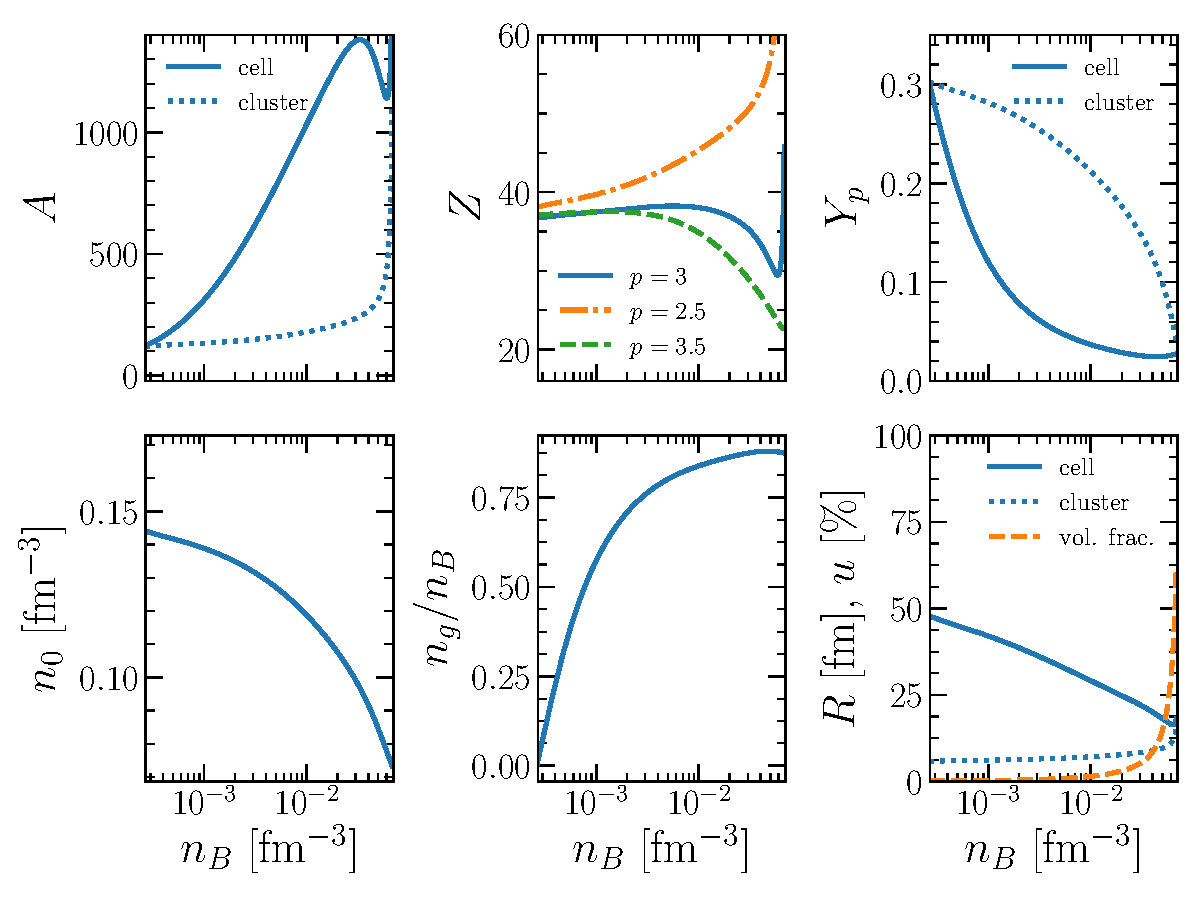
\includegraphics[width=0.9\linewidth]{figures/compo_icrust_bsk24.pdf}
\end{center}
\caption[Ground-state composition versus baryon density in the inner crust]{Variation 
  with baryon density $n_B$ of the equilibrium value of mass 
  number $A$, atomic number $Z$, proton fraction $Y_p$, average cluster density
$n_0$, neutron gas density to baryon density ratio $n_g/n_B$, radius $R$, and
volume fraction $u$ in
the inner crust, for BSk24 CLDM with $p=3$. Solid (dotted) lines correspond to 
the results for the cell (cluster). In the upper-mid panel, three values of the
parameter $p$ are selected: $p=2.5$, $p=3$, and $p=3.5$.}\label{fig:compo_icrust_bsk24}
\end{figure}
%
Fig.~\ref{fig:compo_icrust_bsk24} shows the evolution with baryon density $n_B$ 
of the equilibrium composition of the inner crust. The empirical parameters 
entering in the bulk part of the CLDM energy correspond to the BSk24 effective 
force~\cite{Goriely2013}, and the surface parameter $p$ is fixed at the
educated value $p=3$, which appears to be a reasonable value for Skyrme-type 
functionals, as we will discuss in~\ref{subsec:ccfromc}.
 
It is found that the number of nucleons inside the cluster $A$ as well as inside 
the WS cell $A_{WS}$ monotonously increases with increasing density, going up 
to $\approx 700$ and $\approx 1500$, respectively, at high density. The number 
of free neutrons $N_g = A_{WS} - A$ can also be inferred. It is obviously equal 
to zero at the neutron drip density, since $A=A_{WS}$.
The behavior of $A$ and $A_{WS}$ is in agreement with other CLD calculations, 
such as the one of BBP~\cite{BBP} and that of DH~\cite{Douchin2000a}. The later 
study reports a value of $A \approx 600$ at the CC interface, using the 
SLy4 functional, while BBP report a much higher value of $A=7840$ (see their 
Table 1). Let us notice that the presence of such heavy spherical nuclei at the
crust bottom raises the question of stability with respect to deformation and
fission, as explained in~\cite{Douchin2000a}. In particular, nuclear fission, 
the approximate condition for which is $R_p/R_{WS} \gtrsim
1/2$~\cite{Bohr1939,Pethick1995}, $R_p$ being the
proton radius, could occur at high density. In~\ref{subsec:pasta}, we show that 
considering nonspherical geometries can stabilize the large clusters. It is 
important to stress that the composition, in particular $A$ and $Z$, is very 
sensitive to the isospin dependence of the surface tension at extreme isospin 
ratios. 

The variation with baryon density of the equilibrium value of $Z$ is also 
represented in Fig.~\ref{fig:compo_icrust_bsk24}. We find $Z \approx$ 40 all
along the inner crust with $p=3$, which is in a surprisingly good agreement with 
microscopic results. In particular, in the early work of Negele and Vautherin
(NV)~\cite{Negele1973} is derived a set of nonlinear equations for the single
particle wave functions of nucleons, using the density-matrix expansion for a
realistic NN interaction. NV observed a predominance of $Z=40$ at low density, 
and $Z=50$ at high density. Subsequent works within the semiclassical
ETF~\cite{Goriely2005} and finite-temperature extended Thomas-Fermi plus
Strutinsky integral (TETFSI)~\cite{Onsi2008,Pearson2018} also predict $Z=40$ in
the inner crust. As far as CLD calculations are concerned, DH find that the 
equilibrium value of $Z$ is almost constant in the vicinity of $\approx 40$ 
throughout the inner crust, whereas BBP find monotonically increasing values of $Z$. 
Once again, it should be stress out that $Z$ is very sensitive to the isospin
dependence of the surface tension. In particular, it is observed by varying 
the parameter $p$ that governs the behavior of the surface tension at extreme 
isospin values. We can see that a lower surface tension, $p=3.5$, favors smaller 
atomic number $Z$, and in general lighter clusters, unlike $p=2.5$ that leads to 
heavier clusters.

As in the outer crust, we find that the proton fraction inside the cell $Y_p$ 
continuously decreases in the free neutron regime, dropping from $\approx 0.3$ 
at the neutron drip point to $\approx 0.03$ at the edge of the crust. With
increasing density, clusters also becomes more and more asymmetric, $I$ going
up to $\approx 0.85$ in the bottom layers.

Clusters are found to be more and more dilute with $n_B$ increasing. At the
neutron drip density, we get $n_0 \approx 0.145$ fm$^{-3}$, which is close to the
saturation density of SNM of the BSk24 functional, $n_{sat} = 0.1578$ 
fm$^{-3}$. At the CC interface, the cluster density is as low as $n_0
\approx 0.07$ fm$^{-3}$, which is comparable to the neutron gas density, 
represented is the lower-mid panel. It is seen that the ratio $n_g/n_B$ rapidly
reaches $\approx 75\%$ at $n_B =2\times 10^{-3}$ fm$^{-3}$ then stays
approximately constant at higher densities.

The equilibrium radius of the spherical WS cell $R_{WS}$ and of the spherical 
cluster $R_{cl}$ are also displayed in Fig.~\ref{fig:compo_icrust_bsk24}. As
DH, we observe that $R_{WS}$ monotonically decreases unlike $R_{cl}$ that
slowly increases with increasing depth. Therefore, nuclei becomes closer and closer,
eventually becoming close enough to touch each other at some point, creating a
very large cluster, ultimately leading to homogeneous matter. We can also
understand this by calculating the volume fraction
$u=(R_{cl}/R_{WS})^3 = 2n_p/(n_0(1-I))$ (orange dashed line). We find that the 
cluster fills up to $60\%$ of the WS cell volume at the CC interface. This 
feature combined with the virial theorem, Eq.~(\ref{eq:virial}), outlines the 
fact that lattice and finite-size contributions to the Coulomb energy are 
crucial for the determination of the ground state of the inner crust.

\subsubsection{Equation of state}\label{subsubsec:icrusteos}

\begin{figure}[!t]
\begin{center}
  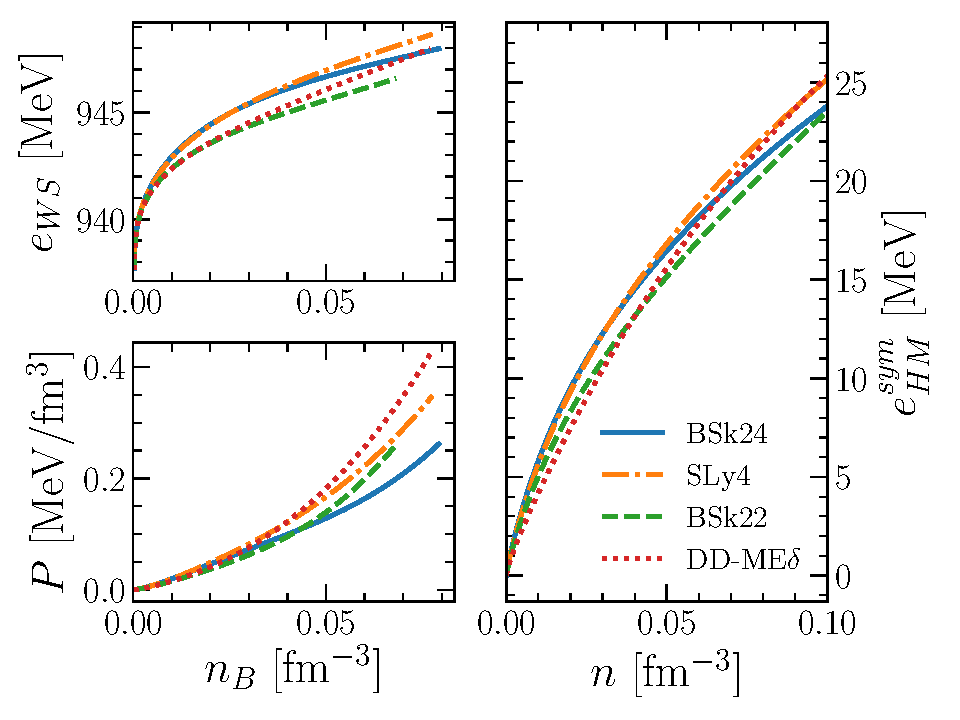
\includegraphics[width=0.9\linewidth]{figures/eos_icrust.pdf}
\end{center}
\caption[Energy per nucleon and pressure versus baryon density in the inner
crust, and symmetry energy at subsaturation densities]{Left: Equilibrium value 
  of the energy per nucleon of the WS cell $e_{WS} =
  E_{WS}/A_{WS}$ (upper panel), and pressure $P$ (lower panel) as a function of 
  the baryon 
density $n_B$ in the inner crust for four selected CLDM: BSk24, SLy4, BSk26,
and DD-ME$\delta$. Right: Variation of symmetry energy $e_{HM}^{sym}$,
Eq.~(\ref{eq:esym_exp}), with density $n$, for the four models.}\label{fig:eos_icrust}
\end{figure}

In Fig.~\ref{fig:eos_icrust}, the equilibrium energy
per nucleon of the WS cell $e_{WS} = E_{WS}/A_{WS}$ is plotted as a function of
the baryon density $n_B$ for different CLDM, based on the relativistic 
model DD-ME$\delta$, and on three Skyrme-type interactions: SLy4, BSk22, and
BSk24. It is observed that $e_{WS}$ depends on the nuclear model. In
particular, it is known to be correlated with the symmetry
energy, with higher symmetry leading to higher $e_{WS}$, at subnuclear
densities~\cite{Pearson2018}. This trend can be verified by looking at the
right panel of the figure, that shows the symmetry energy,
\edit{Eq.~(\ref{eq:esym_exp})}, as a function of density for the four models 
considered here.

Fig.~\ref{fig:eos_icrust} also shows the variation with the 
baryon density of pressure $P$, commonly referred to as the EoS, in the inner
crust. We demonstrate in Appendix \ref{appendix:presic} that the total
pressure, defined by the first law of thermodynamics as
%
\begin{equation}
  P = {n_B^2}\frac{de_{WS}}{dn_B},\label{eq:icpres}
\end{equation}
%
can be expressed as
%
\begin{equation}
  P = P_g + P_e + P_L,
\end{equation}
%
at the equilibrium composition,
where $P_L$ is the lattice contribution to the total pressure. Using this
expression rather than finite differences to estimate the derivative,
Eq.~(\ref{eq:icpres}), is more reliable and has the advantage to be faster from the
computational point of view. In addition, it allows identifying the different
contributions to the pressure. In the inner crust, the pressure is no longer 
dominated by the relativistic electron gas but by the ambient neutron 
gas~\cite{Carreau2017}. At subnuclear densities, we observe that the EoS is 
also correlated with the symmetry energy. In particular, the higher the 
empirical parameter $E_{sym}$, which is the symmetry energy at $n=n_{sat}$, the 
stiffer is the EoS. The value of $E_{sym}$ for each model is reported in
Table~\ref{table:emp_params}.

\subsection{Strutinsky shell corrections to the CLD
energy}\label{subsec:strutinsky}

In the CLD approximation, shell effects, which are known since the pioneering 
work of BPS~\cite{BPS} to be essential to correctly evaluate the outer-crust
composition at zero temperature, are lost.
In this same limit microscopic calculations have shown that the neutron 
shell effects become vanishingly small beyond the neutron drip 
point~\cite{Chamel2006,Chamel2007}, but proton shell effects 
persist in the inner crust.

There are different ways to include shell corrections to the CLD energy. The
simplest approach is to use an empirical formula, such as the one proposed
by Myers and Swiatecki~\cite{Myers1966} which is accurate for reproducing
masses of laboratory nuclei. 
However, a limitation of their method 
is that it requires a priori a list of magic numbers, which are obviously not
known in the regime of the inner crust. Let us recall that NV find a
persistence of $Z=40$ while it is not considered as a magic number in ordinary
nuclei.\\
A more suitable alternative is to calculate shell corrections using the
Strutinsky method \cite{Onsi2008}. 
\edit{Fortunately}, Strutinsky shell corrections \edit{were} calculated 
for modern BSk functionals, and are tabulated in~\cite{Pearson2018} (see
Supplementary data). We therefore add these corrections on top of the CLD 
energy for the corresponding models.

We now turn to the numerical method, proceeding as follows. The energy density
is the quantity to be minimized at constant baryon density for a fixed number 
of protons inside the WS cell. We derive the system of equilibrium 
equations using the Lagrange multipliers method, as in \ref{subsec:formalism}, 
yielding
%
\begin{equation}
  \frac{\partial E_{cl}}{\partial A} - \frac{E_{cl}}{A} = \frac{1-I}{2}
  \left(\mu_e(n_p) +
  \frac{2np}{A(1-I)}\frac{\partial E_{cl}}{\partial n_p} 
  - \frac{2}{A}\frac{\partial E_{cl}}{\partial I} + \Delta
m_{pn}c^2\right),\label{eq:virialthfixz}
\end{equation}
\begin{equation}
  \frac{\partial E_{cl}}{\partial A} + \frac{1-I}{A}\frac{\partial
  E_{cl}}{\partial I} + \frac{P_g(n_g)}{n_0} = \mu_g(n_g) - m_nc^2,
\end{equation}
\begin{equation}
  \frac{n_0^2}{A}\frac{\partial E_{cl}}{\partial n_0} = P_g(n_g).
\end{equation}
%
Let us notice that beta equilibrium is not imposed anymore since $Z$ is fixed, 
causing a modification of Eq.~(\ref{eq:virialthfixz}) with respect to the virial 
theorem with curvature term, Eq.~(\ref{eq:ic1}). For a given $n_B$, the 
minimization is carried out for each tabulated $Z$ using Broyden's 
method. The proton Strutinsky shell corrections are then added perturbatively 
to the CLD energy by interpolation among values of the table, which gives the
shell energy per nucleon for a given $(n_B,Z)$. The WS energy density including
shell corrections thus reads
%
\begin{equation}
  \varepsilon_{WS}(n_B,Z) = \varepsilon_{WS}^{CLD}(n_B,Z) + n_B\Delta
  e_{sh}(n_B,Z),
\end{equation}
%
where $\varepsilon_{WS}^{CLD}$ is the smooth part of the WS energy density at the
equilibrium, and $\Delta e_{sh}$ is the interpolated shell energy per nucleon.
The value of $Z$ that minimizes the energy density of matter is naturally 
defined as the equilibrium value.

\begin{figure}[!t]
\begin{center}
  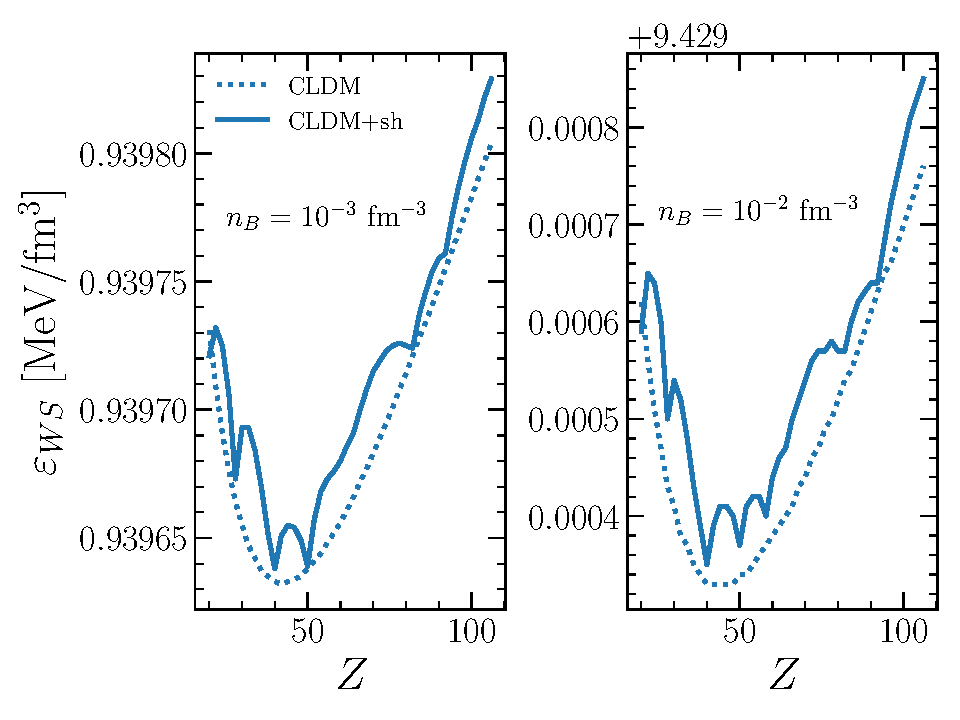
\includegraphics[width=0.9\linewidth]{figures/shcorr_bsk24.pdf}
\end{center}
\caption[Perturbative implementation of proton shell corrections for BSk24]{WS 
  cell energy density as a function of number of protons $Z$ at two
different densities in the inner crust for BSk24 CLDM with (solid lines) and
without (dotted lines) Strutinsky shell corrections on top of the CLD 
energy. \edit{In the right panel, the constant value 9.429 MeV/fm$^3$ is 
  subtracted from the WS cell energy density.}}\label{fig:shcorr_bsk24}
\end{figure}

Fig.~\ref{fig:shcorr_bsk24} shows the variation of the WS energy density as a
function of $Z$ at two selected values of baryon density $n_B$, for BSk24 CLDM. 
As expected, the pure CLD results, represented in dotted lines, are close to 
those including Strutinsky shell corrections, represented in solid lines, for 
closed-shell configurations, while remarkable differences exist for all other 
values of $Z$. This feature confirms the importance of a proper account of the 
shell structure. At $n_B = 10^{-3}$ fm$^{-3}$, a competition between $Z=40$ and
$Z=50$ can be observed, with $Z=40$ being slightly favored. However, it should
be stressed that the difference in energy density is about $10^{-6}$ 
MeV/fm$^{-3}$, which is expected to be lower than the precision reached by our
modeling. It is observed that the shell closure $Z=40$ is also favored over 
$Z=50$ and $Z=58$ at $n_B = 10^{-2}$ fm$^{-3}$.

\begin{figure}[!t]
\begin{center}
  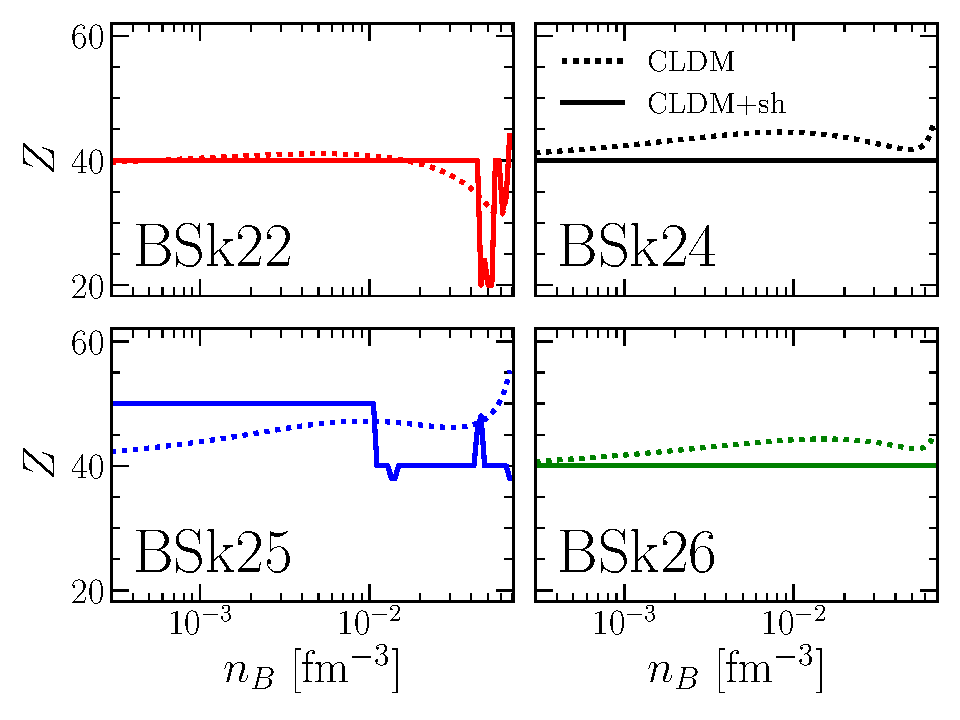
\includegraphics[width=0.9\linewidth]{figures/icrust_compo_bsk.pdf}
\end{center}
\caption[Equilibrium value of $Z$ versus baryon density in the inner crust
with Strutinsky shell corrections]{Equilibrium value of $Z$ as a function of baryon 
  density $n_B$ in the inner crust for BSk22, BSk24, BSk25, and BSk26 CLDM 
  with (solid lines) and without (dotted lines) Strutinsky shell corrections 
  on top of the CLD energy.}\label{fig:icrust_compo_bsk}
\end{figure}

Our results for the equilibrium value of $Z$ in the inner crust using BSk22, 
BSk24, BSk25, and BSk26 CLDM with (solid lines) and without (dotted lines)
Strutinsky shell corrections can be seen in Fig.~\ref{fig:icrust_compo_bsk}.
It can be observed that magic numbers are recovered when shell corrections are
added on top of the CLD energy. In particular, remarkable stability at $Z=40$
is seen for BSk24 and BSk26, as well as $Z=20$ and $Z=40$ for BSk22, in a very 
good agreement with Fig.~12 of~\cite{Pearson2018}. A small difference only
appears for the BSk25 model, reflecting the limitations of the CLD approach.
For this functional, after the plateau at $Z=50$, also obtained with extended
Thomas-Fermi plus Strutinsky integral (ETFSI) calculations
of~\cite{Pearson2018} for the same functional, the equilibrium number of
protons drops to $Z=40$ in our case, instead of increasing as
in~\cite{Pearson2018}. However, we stress that the authors find a second 
minimum at $Z=40$, and the energy difference between the two minima is of 
the order of $10^{-3}$ MeV~\cite{Pearson2019}.

Let us recall that surface and curvature parameters $\sigma_0$, $b_s$, 
$\sigma_{0c}$, and $\beta$ are so far fitted to experimental masses of nearly 
symmetric nuclei from the AME2016~\cite{Huang2017} with a fixed value of the
parameter $p$ that governs the behavior of the surface tension at extreme
isospin values. 
Therefore the shell energy is implicitly accounted for in the surface tension 
by underestimating the value of $\sigma_0$, that is the surface tension of symmetric 
nuclei. This results in predicting slightly overbound nuclei with the CLD
approach, but overall in a better description of spherical nuclei. 
However, we face an issue when adding Strutinsky shell corrections to
the CLD energy, since we do not want to double-count the shell energy. To
address this problem, we fit the surface and curvature parameters to the ETF 
results for each functional~\cite{PearsonPriv}, keeping the parameter $p$ fixed 
to the value $p=3$~\cite{Carreau2019}, which gives an accurate reproduction of 
the CC transition points obtained in~\cite{Pearson2019}.

\subsection{Nonspherical pasta phases}\label{subsec:pasta}

We have assumed so far that the inner crust only consists of spherical 
clusters. However, at high density just before the CC transition, 
nuclei are almost close enough to touch each other, and thus 
the lattice energy significantly reduces the Coulomb energy. Consequently,
matter could in principle arrange itself into exotic structures, sometimes
referred to as nuclear ``pasta''.
In particular, from the density at which the volume fraction exceeds 1/2, it is 
expected that nuclei turn inside out, therefore forming neutron bubbles 
immersed in a proton-rich phase (the former cluster)~\cite{BBP}. Furthermore, 
molecular dynamics simulations, in which a large number of 
interacting nucleons are let evolving in a very large box, predict the appearance of 
complex structures for $Y_p \approx 0.1$, which is comparable to the typical 
value in the bottom layers of the inner crust of neutron 
stars~\cite{Watanabe2003}. It should be stressed that these exotic phases of 
matter could constitute half of the crust mass~\cite{Lorenz1993}. It is
therefore straightforward to imagine that various astrophysical phenomena, such
as the cooling process by neutrino emission, can be affected by 
their existence~\cite{Watanabe2011}.

One of the virtue of the CLD approach is that different geometries for nuclear
clusters can be considered in a simple way, allowing for the study of the pasta
phases~\cite{Ravenhall1983, Lattimer1991, Lorenz1993, Newton2012}. Let us first 
recall the virial theorem with curvature term, here expressed in term of the 
surface, curvature, and Coulomb energy densities,
%
\begin{equation}
  \varepsilon_{surf} + 2\varepsilon_{curv} =
  2\varepsilon_{Coul}.\label{eq:virdens}
\end{equation}
%
Following~\cite{Ravenhall1983,Newton2012}, the general expression for the 
surface energy density is
%
\begin{equation}
  \varepsilon_{surf} = \frac{ud\sigma}{r},
\end{equation}
%
and that of the curvature energy density is
%
\begin{equation}
  \varepsilon_{curv} = \frac{ud(d-1)\sigma_c}{{r}^2},
\end{equation}
%
where the surface tension $\sigma$ and curvature tension $\sigma_c$ are
independent of the dimensionality, and therefore given by 
Eqs.~(\ref{eq:sigma}) and~(\ref{eq:sigmac}), respectively. The Coulomb energy 
density reads
%
\begin{equation}
  \varepsilon_{Coul} = 2\pi(eY_pn_0r)^2u\eta_{Coul,d}(u),
\end{equation}
%
with $\eta_{Coul,2} = \frac{1}{4}\left[\ln\left(\frac{1}{u}\right) + u 
- 1\right]$ for $d=2$, and $\eta_{Coul,d}(u) =
\frac{1}{d+2}\left[\frac{2}{d-2}\left(1-\frac{du^{1-2/d}}{2}\right) +
u\right]$ otherwise.
\\In the previous expressions, $r$ represents the radius (half-width in the
case of planar geometry) of clusters or holes,
$u$ the volume fraction occupied by the cluster (hole), $n_0$ the density of 
the dense phase, and $Y_p$ its associated proton fraction. The expression of 
the volume fraction is different depending on whether we have clusters or 
holes:
%
\begin{equation}
  u =
    \begin{cases}
      (n_B-n_g)/(n_0-n_g) & \text{for clusters,}\\
      (n_0-n_B)/(n_0-n_g) & \text{for holes.}
    \end{cases}       
\end{equation}
%
The parameter $d=\{3,2,1\}$ is related to the dimensionality, 
with $d=3$ for spheres and bubbles, $d=2$ for cylinders and
tubes, and $d=1$ for plates. In the former case, we naturally recover the 
expressions Eqs.~(\ref{eq:esurf}),~(\ref{eq:ecurv}), and~(\ref{eq:ecoul}). Also, let us
note that nuclei and bubble phases are identical as far as plates are concerned.\\
Replacing these quantities in Eq.~(\ref{eq:virdens}), we obtain an equation for
the cluster (hole) radius/half-width,
%
\begin{equation}
  4\pi(eY_pn_0)^2\eta_{Coul,d}(u){r}^4 - d\sigma r - 2d(d-1)\sigma_c 
  = 0,\label{eq:rpasta}
\end{equation}
%
which has to be solved numerically. Let us notice that, neglecting the 
curvature term, the virial theorem reduces 
to $\varepsilon_{surf} = 2\varepsilon_{Coul}$, thus the expression of the 
$r$ is analytical,
%
\begin{equation}
  r =
  \left(\frac{d\sigma}{4\pi(eY_pn_0)^2\eta_{Coul,d}(u)}\right)^{1/3}.
\end{equation}

In order to find the most stable phase at a given baryon density, we proceed as
follows. 
The composition is first calculated at a given $n_B$ in the spherical nuclei 
case ($d=3$) following \ref{subsec:formalism}. Then, keeping the same 
composition, the radius/half-width $r$ is evaluated for the five different 
phases by solving numerically Eq.~(\ref{eq:rpasta}). Finally, since the bulk
and electron contributions to the WS cell are independent of the 
dimensionality, the equilibrium phase is the one that minimizes 
$\varepsilon_{surf} + \varepsilon_{curv} 
+ \varepsilon_{Coul}$. \edit{Let us notice that this method has to be
  considered as an approximation since we do not consider the dimensionality 
  dependence of the surface plus curvature energy in the minimization. This is 
  similar to the so-called ``coexisting phase method'' employed in several 
works \cite{Avancini2008,Avancini2010,Grams2017}.}

\begin{figure}[!t]
\begin{center}
  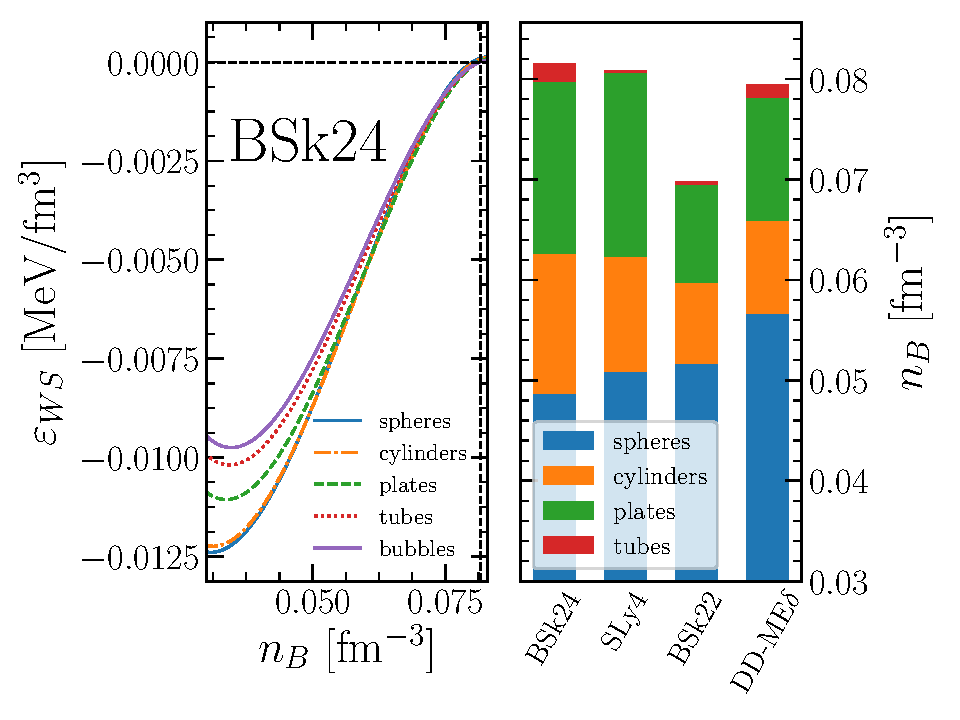
\includegraphics[width=0.9\linewidth]{figures/pasta.pdf}
\end{center}
\caption[Pasta phases in the inner crust]{Left panel: energy density of matter 
  as a function of baryon density for the five phases, using BSk24 
CLDM. The black dashed lines mark the CC transition point. Right panel: 
equilibrium phase as a function of baryon density for four
selected CLDM: BSk24, SLy4, BSk22, and DD-ME$\delta$. For these calculations,
the surface parameter $p$ is fixed to the value $p=3$.}\label{fig:pasta}
\end{figure}

In the left panel of Fig.~\ref{fig:pasta}, we represent the WS energy density
as a function of the baryon density for the five phases, using our CLDM to 
calculate the surface and curvature energy for the BSk24 functional. It is
clearly seen that the spheres dominates up to $n_B \approx 0.05$ fm$^{-3}$,
which is in good agreement with the semiclassical ETF results for this
force~\cite{Pearson2020}. From this density, we find cylinders up to $n_B
\approx 0.065$ fm$^{-3}$, before observing a transition to plates. Then, the
differences in energy density become so small that the possible transition to 
another phase cannot be distinguished in the figure. However, one could expect
the usual sequence, that is a transition to tubes eventually followed by one to 
bubbles before the final transition to homogeneous
matter~\cite{Ravenhall1983}, here marked by the black dashed lines.

The right panel of Fig.~\ref{fig:pasta} shows the equilibrium phase as a
function of $n_B$ for four CLDM: BSk24, SLy4, BSk22, and DD-ME$\delta$. While
model dependence is observed, it is interesting to notice that the 
sequence spheres $\rightarrow$ cylinders $\rightarrow$ plates $\rightarrow$ 
tubes is recovered for every model. Another shared feature is that the 
transition to homogeneous matter is found before the appearance of bubbles.
Let us remark that pasta phases are observed for SLy4 here, while previous CLD 
and TF calculations for this functional have predicted that the sphere is 
the most favorable shape at all densities up to the CC 
transition point~\cite{Douchin2000a, Vinas2017}. This contradiction can be
understood by the fact that we are dealing with very tiny differences in
energy density (all the shapes are very close), in a region where the matter is 
extremely neutron rich, thus
where the nuclear surface tension is poorly constrained. In particular, we 
observed that varying the value of the surface parameter $p$ can affect the 
sequence of pasta phases.

\subsection{Crust-core transition from the crust side}\label{subsec:ccfromc}

It is well known that a phase transition from a solid crust to a liquid core
takes place at some $\approx 1$ km from the surface of the star, corresponding 
to subsaturation densities. A precise estimation of this transition point is 
necessary in order to evaluate the crust mass, thickness and moment of inertia, 
and so to understand phenomena involving NS, such as glitches, that are 
irregularities in the their rotational motion~\cite{Espinoza2011}. In that 
sense, a Bayesian analysis of the CC transition has been 
performed~\cite{Carreau2019cc} and is presented in details in Chapter 2. 

The simplest approach for computing the phase transition is from the core side, 
in which the transition is defined as the density point where homogeneous 
nuclear matter (NM) at beta equilibrium becomes unstable with respect to 
density fluctuations. Two versions of this technique can be distinguished: the 
so-called thermodynamical \cite{Gonzalez2017} and 
dynamical \cite{Pethick1995cc,Antic2019} methods.\\
The former method consists in evaluating the thermodynamical spinodal, that is 
the instability point of NM with respect to the liquid-gas (LG) phase 
transition. The only necessary nuclear physics input for this method is the 
energy functional of homogeneous NM, which can is well constrained through
nuclear experiments and/or ab initio calculations in the vicinity of the
nuclear saturation density $n_{sat}$. While it appears as a substantial 
advantage, it is known that the dynamics of the CC transition is very different 
from the LG one~\cite{Ducoin2007a,Ducoin2007b,Ducoin2008}, thus applying this 
method results in an overestimation of the 
CC transition density and pressure. Indeed, the CC transition is expected 
to take place at approximately $\approx n_{sat}/2$, where the energy density of 
clusterized matter overcomes that of uniform NM~\cite{BBP}. Since Coulomb, surface,
and curvature terms, that are crucial for determining the equilibrium
composition in the inner crust, vanish in homogeneous NM, they no not 
contribute to the determination of the LG thermodynamical spinodal.\\
In the dynamical method, finite-size density fluctuations are added, thus 
it is expected to give a better estimation of the CC transition and pressure. 
It should be stressed that the isovector gradient terms, which are needed in
addition to the EoS with respect to the thermodynamical method, play a 
nonnegligible role for the determination of the dynamical spinodal, the
location of which also depends on the many-body formalism 
adopted~\cite{Ducoin2008}.

While the dynamical method gives a better estimation of the CC transition point
in comparison with the thermodynamical one, one should remark that the spinodal
decomposition scenario is not compatible with the equilibrated crust in which
matter is not uniform but composed of clusters immersed in a sea of electrons
and neutrons. For this reason, the CC transition point is here computed from 
the crust side, by comparing the energy density of the two competing phases in 
beta equilibrium. The equation for the CC transition density $n_t$ is thus
%
\begin{equation}
  \varepsilon_{WS}^{crust}(n_t) = \varepsilon_{npe}(n_t),\label{eq:cctp}
\end{equation}
%
where $\varepsilon_{WS}^{crust}$ is the equilibrium energy density in the WS
cell in the inner crust, and $\varepsilon_{npe}$ is the equilibrium energy
density of matter in the outer core, which consists of homogeneous \textit{npe} 
matter, studied in Section~\ref{sec:core}.
The CC transition point is computed in the following for several nuclear 
models, using the metamodeling technique extended to finite nuclei in the 
CLD approximation, Eq.~(\ref{eq:enuc}), to calculate the WS cell energy density in 
the inner crust, and keeping the same empirical matter for the description of 
uniform \textit{npe} matter. One should stress the importance of having a 
unified EoS for the crust and the core~\cite{Douchin2001} to estimate correctly 
the CC transition point. Indeed, it was shown that matching a crust and core
EoS based on different nuclear models induce an uncertainty on the determination 
of the CC transition point, consequently inducing an uncertainty in the crustal 
observables, which can be as large as $30\%$ for the crust
thickness~\cite{Fortin2016}.\\
Let us mention that pasta phases are not 
considered here, since we have checked that their presence does not 
affect the estimation of the CC transition density and pressure.

\begin{figure}[!t]
\begin{center}
  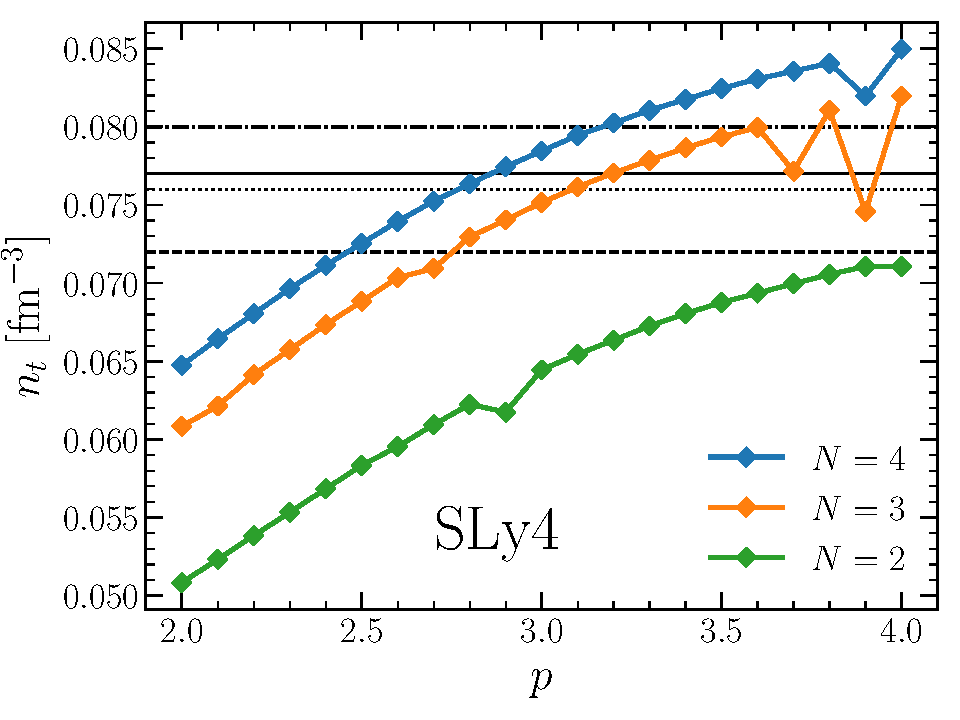
\includegraphics[width=0.8\linewidth]{figures/sly4_nt.pdf}
\end{center}
\caption[Crust-core transition density versus surface parameter $p$ for SLy4]{Crust-core 
  transition density as a function of the surface parameter  
$p$ with truncation order $N=2$, $N=3$, and $N=4$, for SLy4 CLDM. The black
horizontal bars represent different evaluations of $n_t$ for the SLy4
functional found in the literature: $n_t=0.072$ fm$^{-3}$ \cite{Vinas2017}
(dashed line) and $n_t=0.077$ fm$^{-3}$ \cite{Douchin2000a} (solid line) in the
CLDM approximation, $n_t=0.076$ fm$^{-3}$ \cite{Vinas2017} (dotted line) in the
TF approximation, and $n_t=0.080$ fm$^{-3}$ \cite{Vinas2017} (dashdotted line)
with the dynamical method.}\label{fig:sly4_nt}
\end{figure}

In Fig.~\ref{fig:sly4_nt}, we show the variation with surface parameter $p$ of 
$n_t$ for SLy4 CLDM. For each value of $p$, the surface and curvature 
parameters are fitted to experimental masses from the AME2016. 
The CC transition density is estimated for different 
values of the truncation order $N$ in the density development, 
Eq.~(\ref{eq:mm}). A convergence feature is observed from $N=2$ to $N=4$,
almost achieved at $N=3$. We can see that truncating at $N=2$ leads to a 
substantial underestimation of about $\approx 20\%$ of the transition density. 
This observation highlights the importance of keeping high-order 
parameters beyond $(Q_{sat},Q_{sym})$ ($N=3$), and $(Z_{sat},Z_{sym})$ ($N=4$)
in the Taylor expansion.\\
A positive correlation is seen between the isovector surface parameter $p$ and 
$n_t$: the higher the value of $p$ the higher the transition density. This can 
be understood from the fact that a low value of $p$ leads to a higher surface 
tension at extreme isospin values, thus it makes the cluster less bound and
consequently the uniform ${npe}$ matter becomes the favorable phase at lower
density.\\
Different estimations of the CC transition density for the SLy4 functional
found in the literature are reported in Fig.~\ref{fig:sly4_nt} (black lines), 
with $n_t$ ranging from 0.072 fm$^{-3}$ \cite{Vinas2017}, in the 
CLD approximation, to 0.089 fm$^{-3}$ \cite{Ducoin2011} (not represented in the 
figure), with the thermodynamical method. It is interesting to observe that 
the \edit{two different} CLDM calculations \edit{of the literature based on
SLy4 functional, reported in the figure}, give a different estimation of 
$n_t$, with 0.072 fm$^{-3}$ in~\cite{Vinas2017}, and 0.077 fm$^{-3}$ 
in~\cite{Douchin2000a}. This stresses once again the importance of the 
treatment of the isovector surface tension for the determination of the CC 
transition point.\\
The effect of the varying the low-density parameter $b$ on $n_t$ is also 
evaluated in \cite{Carreau2019cc}. It is found that while it does not 
significantly affect the transition density in comparison with $N$ and $p$, it 
should be kept as an additional EoS parameter in any statistical analysis in
order to make a quantitative prediction of the CC transition point.
\edit{The introduction of the parameter $b$ in the parameter space is, in fact, 
  an effective manner to account for the effect of orders $N>4$, which is not 
important.}

\begin{figure}[!t]
\begin{center}
  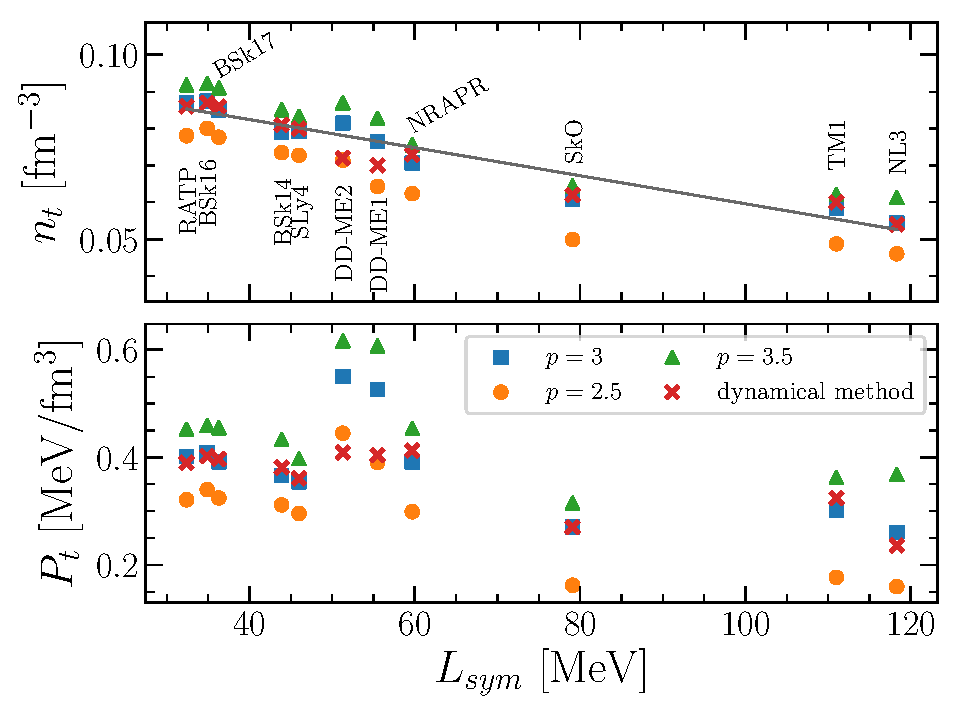
\includegraphics[width=0.9\linewidth]{figures/cctp_lsym.pdf}
\end{center}
\caption[Crust-core transition density and pressure for several interactions]{Crust-core 
  transition density $n_t$ (upper panel) and pressure $P_t$ 
(lower panel) as a function of $L_{sym}$ for several interactions. The crosses 
are the transition points calculated in \cite{Ducoin2011} using the dynamical
spinodal. The circles, squares, and triangles correspond respectively to our
estimation of the transition points with $p=2.5$, $p=3$, 
and $p=3.5$. The gray line is the linear regression curve fitted to the $p=3$ 
results.}\label{fig:cctp_lsym}
\end{figure}

Fig.~\ref{fig:cctp_lsym} shows our estimations of the transition density $n_t$ 
and pressure $P_t$ as a function of the slope of the symmetry energy $L_{sym}$ 
for a set of relativistic and nonrelativistic functionals, in 
comparison with the dynamical spinodal calculations of \cite{Ducoin2011}. It is
seen that the value $p=3$ is in good agreement with the dynamical results for
most of the models. For DD-ME2, the lower value needed for $p$ is supported by
the TF calculations in \cite{Grill2012}.\\
As in~\cite{Vinas2017}, an anticorrelation is observed between $L_{sym}$ and 
$n_t$. Using a linear regression to model the relationship between $L_{sym}$
and our estimation of $n_t$ with $p=3$, we find $n_t = -3.807\times
10^{-4}L_{sym} + 0.098$ fm$^{-3}$, for a root mean square error of 
$3.094\times 10^{-3}$ fm$^{-3}$. This is linear equation for $n_t$ is in very
good agreement with Eq.~(17) of \cite{Ducoin2011}.
This downwards tendency with increasing values of $L_{sym}$ is not clearly 
observed for the transition pressure. \edit{We will see in Chapter 2 that the 
  relation between those two quantities is less explicit because $P_t$ rather 
  depends on $K_{sym}$, which is logical because the pressure requires the
  calculation of one more derivative in comparison to the energy density that 
defines $n_t$.}

% -----------------------------------------------------------------------------

\section{Matter of the core}\label{sec:core}

In the very bottom layers of the inner crust, clusters are so large and
asymmetric that the CLD energy per nucleon, Eq.~(\ref{eq:enuc}), becomes equal to 
that of infinite nuclear matter, marking the CC interface. While the
composition and structure of the core close to the saturation density are well
known, various scenarios have been proposed in the
literature~\cite{Oertel2017} concerning the relevant degrees of freedom 
above $2-3n_{sat}$. 

This section deals with the matter of the core. In \ref{subsec:ocore} we derive
the system of variational equations for the ground state of the outer core. The
model dependence of the composition and EoS is then explored. In particular, we
focus on apparent correlations with the symmetry energy. The matter inside the 
inner core is finally discussed in \ref{subsec:icore}.

\subsection{Outer core: homogeneous \textit{npe$\mu$}
matter}\label{subsec:ocore}

From the CC transition point, previously discussed in~\ref{subsec:ccfromc}, up to 
$n_B \approx 2n_{sat}$, the matter of the core consists of a uniform plasma of 
neutrons, protons, electrons, and eventually muons, hereafter referred to 
as \textit{npe$\mu$} matter (or \textit{npe} if muons are not
present). This region of the star corresponds to the outer core.
The energy density of \textit{npe$\mu$} matter reads
%
\begin{equation}
  \varepsilon_{npe\mu}(n_B,\delta,n_e,n_{\mu}) = \varepsilon_{HM}(n_B,\delta) +
  \varepsilon_{e}(n_e) + \varepsilon_{\mu}(n_{\mu}) + n_B\frac{1-\delta}{2}\Delta
  m_{pn}c^2 + n_B m_n c^2,\label{eq:epscore}
\end{equation}
%
with $\varepsilon_{HM} = ne_{HM}$ the energy density of nuclear matter 
given by the metamodel, Eq.~(\ref{eq:meta}). The expression of energy density
of the relativistic muon gas $\varepsilon_{\mu}(n_{\mu})$ is the same as that 
of the relativistic electron gas, and it is derived in Appendix \ref{appendix:epse}.

\subsubsection{Variational equations}

Following~\ref{subsec:formalism}, the system of differential equations
determining the equilibrium composition and EoS in the outer core is
determined by minimizing the energy density of matter, Eq.~(\ref{eq:epscore}), 
at constant baryon density under the condition of overall charge neutrality, 
which now reads
%
\begin{equation}
  n_B\frac{1-\delta}{2} = n_e + n_{\mu}.\label{eq:chargecon}
\end{equation} 
%
since muons may exist in this region of the star. Muons are present in
the outer core if the electron chemical potential exceeds the muon rest-mass 
energy, that is $\mu_e \gtrsim m_\mu c^2$.\\
As far as variational variables are concerned, a reasonable choice appears to
be the asymmetry $\delta$ and the muon density $n_{\mu}$. Let us first minimize
the energy density of matter with respect to $\delta$,
%
\begin{eqnarray}
  \frac{\partial \varepsilon_{npe\mu}}{\partial \delta}\bigg|_{n_\mu} &=&
  0\notag \\
  2\frac{\partial e_{HM}}{\partial \delta} - \Delta m_{pn}c^2 - \mu_e &=& 0.
\end{eqnarray}
%
We can easily identify this equation with the well-known beta equilibrium 
condition. Indeed, using the definition of the neutron and proton chemical 
potentials, Eq.~(\ref{eq:chempot}), we obtain
%
\begin{equation}
  \mu_n = \mu_p + \mu_e.\label{eq:betaeqcore}
\end{equation}
%
We now turn to minimization with respect to the muon density,
%
\begin{eqnarray}
  \frac{\partial \varepsilon_{npe\mu}}{\partial n_{\mu}}\bigg|_{\delta} &=&
  0\notag\\
  \mu_{\mu} - \mu_e &=& 0,\label{eq:muemumu}
\end{eqnarray}
%
where we have introduced the muon chemical potential $\mu_\mu = \partial
\varepsilon_\mu/\partial n_\mu$. This equation corresponds to the chemical 
equilibrium between muons and electrons, and has to be satisfied if muons are 
present. These two equations, Eq.~(\ref{eq:betaeqcore}) and~(\ref{eq:muemumu}), 
express the equilibrium with respect to the weak interaction processes. 
\edit{Let us remark that each time we mention electrons and muons, we are always 
  referring to their net number, that is particles minus antiparticles.}

% explain numerically
From the numerical point of view, we use Broyden's method to solve the beta
equilibrium equation, Eq.~(\ref{eq:betaeqcore}), starting from the transition 
density $n_t$. The initial guess for the asymmetry $\delta_{guess}$ is taken to be 
the value of the global asymmetry inside the WS cell at the CC transition 
point, which is approximately $\approx 0.9$. At each new step of baryon 
density, the value of 
$\delta_{guess}$ is updated with the last equilibrium solution, and we check
if $\mu_e \gtrsim m_\mu c^2$. In the case of \textit{npe$\mu$} being
energetically favorable, Eq.~(\ref{eq:muemumu}) is added as a supplementary
equation to be solved, setting the initial guess for the muon density to
$n_{\mu,guess} = 10^{-5}$ fm$^{-3}$.  The calculation is stopped when the 
baryon density reach $\approx 2n_{sat}$, from which the composition of matter 
becomes less certain.

\subsubsection{Equilibrium composition and equation of state}

\begin{figure}[!t]
\begin{center}
  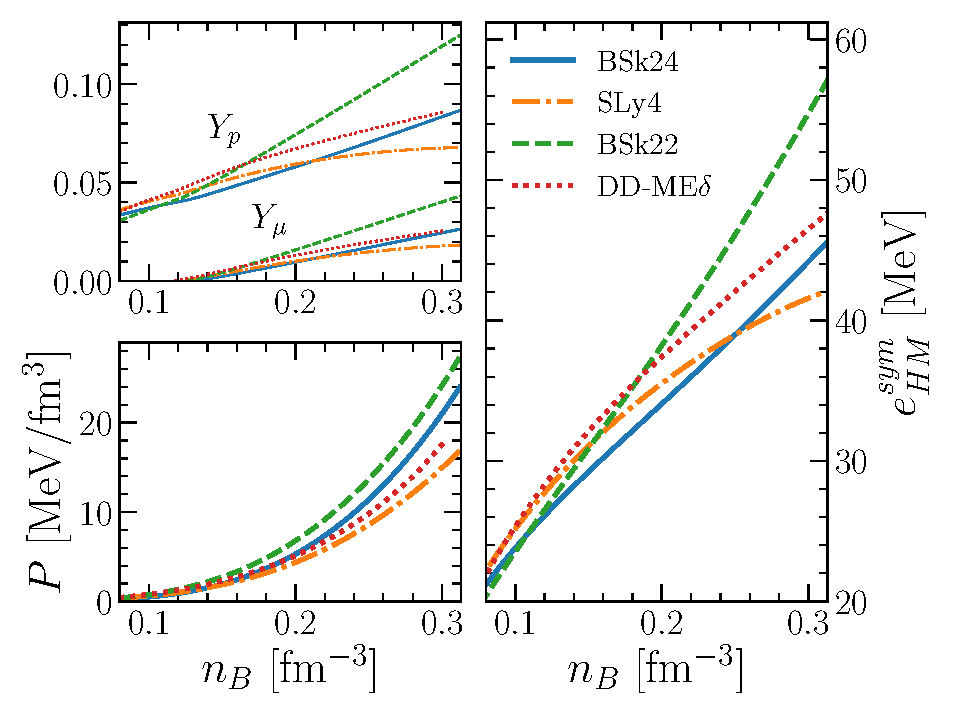
\includegraphics[width=0.9\linewidth]{figures/ocore.pdf}
\end{center}
\caption[Equilibrium composition, pressure, and symmetry energy versus baryon
density in the outer core]{Left: Proton fraction $Y_p$ and muon fraction 
  $Y_\mu$ (upper panel), and pressure $P$ (lower panel) as a function of the 
  baryon density $n_B$ in the outer core for four selected models: BSk24, SLy4, 
  BSk22, and DD-ME$\delta$. Right: Variation with baryon density of the symmetry 
energy $e_{HM}^{sym}$, Eq.~(\ref{eq:esym_exp}), for the four 
models.}\label{fig:ocore}
\end{figure}

In Fig.~\ref{fig:ocore}, the proton fraction $Y_p=(1-\delta)/2$ and muon 
fraction $Y_\mu = n_\mu/n_B$ are plotted as a function of the baryon density 
for the four nuclear models BSk24, SLy4, BSk22, and DD-ME$\delta$, the
empirical parameters of which are listed in Table~\ref{table:emp_params}. The
variation $n_B$ of the electron fraction $Y_e$ can be deduced from the
charge neutrality condition, Eq.~(\ref{eq:chargecon}). Surprisingly, it is
observed that the proton fraction rises with $n_B$ in the outer core, while 
it monotonously decreases in the crust. 
A strong correlation between the proton fraction and the symmetry energy,
represented in the right panel for the four models, is seen. One can relate the 
two quantities using the beta equilibrium condition. Indeed, we can easily go 
through Eq.~(\ref{eq:betaeqcore}) assuming a quadratic expansion for the NM 
energy per nucleon,
%
\begin{equation}
  e_{HM}(n_B,\delta) \simeq e_{HM}(n_B,\delta=0) + \delta^2 e_{HM}^{sym}(n_B).
\end{equation}
%
In that case, the beta equilibrium condition reads
%
\begin{equation}
  4\delta e_{HM}^{sym}(n_B) - \Delta m_{pn}c^2 = \mu_e(n_e),
\end{equation}
%
and we can thus express the proton equilibrium proton fraction as a function of 
the symmetry energy,
%
\begin{equation}
  Y_p = \frac{1}{2} - \frac{\mu_e(n_e) 
  + \Delta m_{pn}c^2}{8e_{HM}^{sym}(n_B)}.
\end{equation}
%
From this equation it is clear that the higher the symmetry energy, the higher
the proton fraction, which is the trend observed in the figure.\\
The density from which muons are present is also shown in the upper left
panel. It appears that we are dealing with \textit{npe} matter up to 
$n_B \approx 0.12$ fm$^{-3}$, and it is seen that the threshold density for the
appearance of muons, when $\mu_e \gtrsim m_\mu c^2$, is not very sensitive to 
the nuclear model.

Fig.~\ref{fig:ocore} also shows the pressure as a function of the density
(lower left panel). In the outer core, we can write the pressure as
%
\begin{equation}
  P(n_B) = P_{HM}(n_B, \delta) + P_e(n_e) + P_\mu(n_\mu),
\end{equation}
%
where $\delta$, $n_e$, and $n_\mu$ are the equilibrium values at $n_B$. The
expression of the nuclear contribution $P_{HM}$ is given by
Eq.~(\ref{eq:phm}). The electron and muon contributions to the total pressure, 
respectively $P_e$ and $P_\mu$, share the same expression, Eq.~(\ref{eq:pel}), 
which is that of a relativistic Fermi gas. A strong model dependence is
observed for the pressure at suprasaturation densities, reflecting the large
uncertainties associated to the isovector parameters beyond $E_{sym}$, as
reported in the last column of Table~\ref{table:emp_params}.

\subsection{Inner core}\label{subsec:icore}

From the crust-core interface up to $n_B \approx 2n_{sat}$, it is commonly
accepted that matter is exclusively composed of neutrons, protons, electrons, 
and muons. At higher densities however, the composition of matter becomes
uncertain and different scenarios have been considered in the
literature for the structure and composition of the inner 
core \cite{Oertel2017}. The presence of hyperons at suprasaturation densities 
has been considered in many studies, and its effect on the EoS and 
subsequently on NS observables has been 
evaluated \cite{Bednarek2012,Fortin2015}. In particular, the 
presence of hyperons softens the high-density EoS and thus lowers the maximum 
mass of neutron stars. As a consequence, many models fail to satisfy the NS 
mass constraint of $\approx 2M_\odot$~\cite{Demorest2010,Antoniadis2013}, 
leading to the so-called ``hyperon puzzle''~\cite{Zdunik2013}. In fact, the 
measurement of $\approx 2M_\odot$ NS also rules out most of the models that 
include a phase transition to quark matter or a boson condensate in the inner 
core, because the EoS is softened
by the introduction of any additional degree of freedom without an 
interaction. Let us however mention a recently proposed EoS with a 
quark-hadron crossover at high density that allows a maximum mass of 
$2.35M_\odot$ \cite{Baym2019} and agrees with the constraints on NS
properties inferred from the GW170817 event \cite{GW1,GW2}.

We propose here to extrapolate the \textit{npe$\mu$} matter at higher
densities, in the inner core. \edit{The different studies that consider 
  hyperons and satisfy the maximum mass 
constraint show that the hyperon-nucleon and hyperon-hyperon are such 
that, if hyperons exist, they are not abundant and can be neglected as a first 
approximation, at least in the EoS energetics (see \cite{Oertel2017} and
references therein). Since the metamodeling does not make any assumption 
regarding the degrees of freedom, but that the functional is based on a Taylor 
expansion, we can assume that the technique can be safely extended at high 
density in the aim of calculating static properties, such as the EoS or the 
mass-radius relation. The only thing that could invalidate it would be the 
presence of a large first-order phase transition, that is a large discontinuity 
in the EoS. Thus, the only hypothesis that is made here is considering that 
there is no such transition. Actually, even a transition to quark matter could 
be smooth. Indeed, several works consider pasta phases in the hadron-quark 
phase transition, with the effect of washing out
discontinuities \cite{Maruyama2009,Yasutake2009,Yasutake2011,Yasutake2014}. 
Finally, this is equivalent to a null hypothesis: since the metamodeling 
allows to control uncertainties, a disagreement with astrophysical 
observations would be the sign of new physics, indicating either the existence
of a first-order phase transition or an alternative theory of gravity.} Let us 
recall that the metamodeling technique gives an accurate reproduction of
existing nuclear models up to $\approx 2-3 n_{sat}$ (metamodeling ELFc 
in \cite{Margueron2018a}), as we have verified in Fig.~\ref{fig:mm_accuracy}.
A solution for achieving faster convergence at high density, the 
metamodeling ELFd, is proposed in \cite{Margueron2018a}. It is based on a
reevaluation of the high-order empirical parameters parameters $Q_{sat}$,
$Q_{sym}$, and $Z_{sat}$, $Z_{sym}$, by imposing a high-density point at which
the energy per nucleon and the pressure are known for a given functional. This
is encouraged by the fact that the impact of these parameters is very small in
the vicinity of the saturation density. We will use this technique when we will
want to reproduce existing hadronic models.

% -----------------------------------------------------------------------------

\section{Unified metamodeling of the equation of state}\label{sec:mmeos}

\begin{figure}[!t]
\begin{center}
  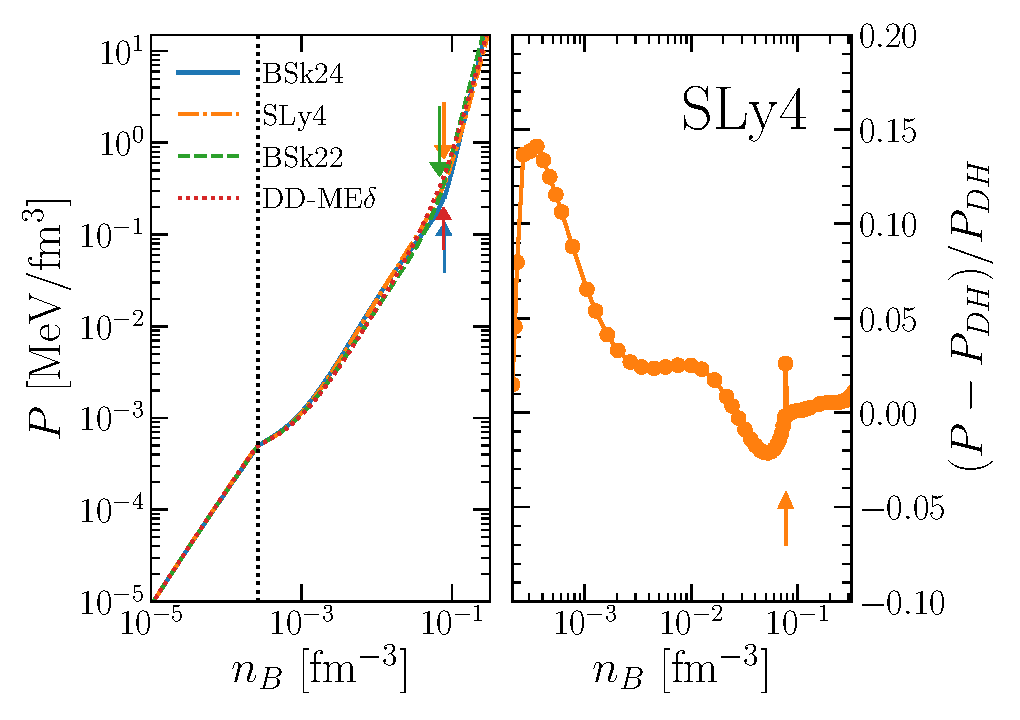
\includegraphics[width=0.9\linewidth]{figures/unified.pdf}
\end{center}
\caption[Unified metamodeling of the equation of state]{Left: Pressure as a
function of baryon density in the different regions of a NS for BSk24, SLy4,
BSk22, and DD-ME$\delta$. Crust and core are described in a unified manner, 
with the metamodeling technique. The black dotted line marks the onset of the 
inner crust, and arrows indicate the CC transition density for the
different models. Right: Relative difference $(P - P_{DH})/P_{DH}$ with 
DH unified EoS for SLy4~\cite{Douchin2001} as a function 
of $n_B$. The arrow indicates our estimation of the CC transition 
density for SLy4.}\label{fig:unified}
\end{figure}

As previously discussed, matching a crust and core based on different nuclear
models can lead to large uncertainties associated with the CC transition
density and pressure, which are the quantities for the determination of the
crust observables. In particular, it was shown in \cite{Fortin2016} that it 
can lead to an error as large as $\approx 30\%$ for the crust thickness and
$\approx 4\%$ for the radius. The main justification for working with nonunified 
EoS is that the core is responsible of most of the NS mass, thus one could 
simply match any crust EoS, for instance that of BPS in the outer 
crust~\cite{BPS} plus that of BBP in the inner crust~\cite{BBP}, 
with its core EoS based on a different nuclear interaction. This is indeed 
sufficient if one is interested in observables such as the maximum mass. 
However, it obviously leaves a large freedom in the matching procedure. In 
addition, this amounts to consider that the crust segment is not model 
dependent, while we have clearly 
seen in \ref{subsubsec:icrusteos} that the crust EoS is sensitive to the 
nuclear model, and is in particular correlated with the symmetry energy. It 
is therefore preferable to describe the crust and core in a unified 
manner.

Several unified EoS for cold non-accreting NS have been proposed in the 
literature. For instance, the 
well-known DH EoS~\cite{Douchin2001} is based on the Skyrme SLy4 effective
interaction~\cite{Chabanat1998}. In the inner crust, the authors use a version 
of the CLDM to calculate the energy of finite nuclei, the bulk term of which is 
given by the SLy4 functional in the infinite NM limit, which is also used to 
describe the outside neutron gas, and at high density to calculate 
the \textit{npe$\mu$} matter energetics in the core. Let us notice that the EoS
of the outer-crust ground state is taken from~\cite{Haensel1994} in this 
work.\\
More recently, a series of unified EoS based on modern BSk 
functionals~\cite{Goriely2013} has been proposed~\cite{Pearson2018}. In this
work, the ground state of the outer crust is determined by application of the
microscopic HFB method~\cite{Samyn2002}, and the ground state of the inner 
crust is calculated within the ETFSI approximation~\cite{Onsi2008}. \edit{Also, 
  a set of unified EoS were built within a relativistic mean-field approach 
(RMF) in \cite{Fortin2016}.}

One obvious reason explaining why crust and core matter are not consistently 
treated using the same microscopic interaction is that it is less trivial to 
evaluate the ground state of the inner crust in comparison to the ground state
of matter in the core. Indeed, one can evaluate the inner-crust ground state
within different many-body approaches, either using the CLDM, the
semiclassical ETFSI method, or full HF calculations. While 
the two last methods are expected to be more precise with respect to the CLD 
approximation as far as the composition is concerned, they can become 
computationally heavy if one wants to compute the EoS for many nuclear 
models. \edit{In addition, these more microscopic methods can only be extended 
  to finite temperature in the SNA, whereas the CLD approximation allows 
distributions of clusters, that exist at $T > 0$, to be considered.} \\
In view to provide a unified and thermodynamically consistent treatment of the
crust and core of cold non-accreting NS, we propose to compute the EoS within 
the metamodeling approach that we have presented throughout this chapter. For
a given nuclear model, in other words a given set of empirical parameters
$\bm{P_\alpha}$, we proceed as follows. The EoS in the outer crust is
evaluated by application of the BPS method presented in \ref{subsec:bps}, using 
the present day knowledge on experimental masses~\cite{Huang2017} supplemented 
by state-of-the-art microscopic HFB theoretical mass tables~\cite{Goriely2013} 
up to the neutron-drip point. The EoS in the inner crust is then calculated
by solving the system of four differential equations, Eqs.~(\ref{eq:ic1}),
(\ref{eq:ic2}), (\ref{eq:ic3}), and (\ref{eq:ic4}). The metamodeling technique,
discussed in ~\ref{subsubsec:hnm}, is used to calculate the neutron gas energy.
The concept of metamodeling of homogeneous NM is extended to finite nuclei in the
CLD approximation in order to evaluate the cluster energy, the bulk term of
which is calculated with the same empirical parameters as the neutron gas. 
Finally, from the CC transition point, discussed in~\ref{subsec:ccfromc}, the 
core EoS is computed by solving the two chemical equilibrium equations
Eqs.~(\ref{eq:betaeqcore}) and~(\ref{eq:muemumu}). Again, the empirical
parameters are the same as those used in the inner crust. Within such an 
approach, one can compute the unified EoS for any nuclear model.
In addition, this method is not expensive from the computational point of view,
which will allow us to make comprehensive statistical evaluations of the model
uncertainties in Chapter 2. 

The left panel of Fig.~\ref{fig:unified} shows the resulting unified EoS for
the four nuclear models considered in this chapter: BSk24, SLy4, BSk22, 
and DD-ME$\delta$. The neutron-drip point is represented by the vertical dotted
line, and arrows indicate the CC transition density for each model.\\
The relative difference between the DH EoS~\cite{Douchin2001} and our EoS for
SLy4 is represented as a function of the baryon density in the right panel of
Fig.~\ref{fig:unified}. It is seen that the overall difference is smaller than 
$10\%$ in the inner crust. The slight disagreement at low density comes from 
the fact that the onset of the inner crust is marked at $n_{ND} = 2.0905 \times
10^{-4}$ fm$^{-3}$ in the DH EoS (calculated in \cite{Haensel1994}), which is 
low in comparison with our estimation of the neutron drip density, $n_{ND} = 
2.503\times 10^{-4}$ fm$^{-3}$. Let us notice that the parametrization of the
surface tension in both studies is different, therefore it might explain the 
difference between the two EoS at higher densities in the inner crust, in 
addition to the slight error introduced by the metamodel. In the core, we can
observe that the relative difference is smaller that $1\%$.

% -----------------------------------------------------------------------------

\section{Conclusion}\label{sec:conclu1}

In this chapter, we have first evaluated the ground state of the outer crust, 
which is obtained by the application of the BPS method, using recent 
experimental masses~\cite{Huang2017,Welker2017} supplemented by state-of-the-art 
microscopic HFB theoretical mass tables. We have shown that the outer-crust 
composition and so the EoS are entirely determined by the present day
knowledge on experimental masses up to $n_B \approx 3\times 10^{-5}$ fm$^{-3}$.
At higher densities, we have observed the persistence of $N=82$ for each of the
four mass models considered.

We have proposed a version of the CLDM based on the metamodeling
technique \cite{Margueron2018a,Margueron2018b}. We have seen that the
metamodel offers the possibility to reproduce any functional of nuclear matter 
very precisely, \edit{with a unique functional form}. The parametrization of 
surface tension was suggested from
microscopic calculations in the free neutron regime~\cite{Ravenhall1983}, and
surface and curvature parameters are fitted to experimental masses. We have used 
the CLDM to calculate the ground state of the inner crust, which is obtained by
minimizing the energy density of matter at constant baryon density under the
condition of overall charge neutrality. We have therefore derived a system of
four coupled differential equations, corresponding to chemical and mechanical
equilibrium conditions, that we have solved numerically using Broyden's method.
The ground-state composition of the inner crust for BSk24 empirical parameters 
was presented, and a very good agreement with more microscopic approaches was 
observed concerning the value of $Z \approx 40$. We have also seen that the 
proton fraction is continuously decreasing, as in the outer crust. The inner
crust EoS was computed and a positive correlation with the empirical 
parameter $E_{sym}$ was revealed. We have shown that magic numbers, that vanish
within the CLD approach, can be recovered by adding perturbatively Strutinsky
shell corrections on top of the CLD energy. In this way, a very good agreement 
with ETFSI calculations was observed for recent BSk 
functionals \cite{Pearson2018}. With the CLDM, we have explored the possible 
presence of nonspherical pasta phases in the bottom layers of the inner crust,
finding the sequence spheres $\rightarrow$ cylinders $\rightarrow$ plates
$\rightarrow$ tubes for each of the four model considered: BSk24, SLy4, BSk22,
and DD-ME$\delta$. We have shown that the transition point to homogeneous
matter is very sensitive to the surface tension at extreme values of isospin, 
the behavior of which is governed by the isovector surface parameter $p$.
Unfortunately, this parameter cannot be accessed from empirical nuclear physics 
data, which are limited to values around $I \lesssim 0.3$. We have seen that 
the CC transition density and pressure results of the literature for the 
dynamical spinodal~\cite{Ducoin2011} are globally nicely reproduced by our 
calculation from the crust with $p \approx 3$. We have also confirmed
the correlation of the transition density $n_t$ with the empirical parameter
$L_{sym}$ already observed in previous works.

We have derived the equilibrium equations characterizing the ground state of
matter in the core, which consists of \textit{npe$\mu$} matter up to $n_B
\approx 2n_{sat}$. The strong correlation between the symmetry energy and the 
proton fraction was explained. We have found that muons appear in the vicinity 
of $n_B \approx 0.12$ fm$^{-3}$ for each model. As in previous works
\cite{Wiringa1988,Douchin2001}, we have extrapolated the npe$\mu$ model to 
higher densities, since the hyperon-hyperon and hyperon-nucleon interactions 
remain currently poorly constrained.

Finally, we have stressed that building unified EoS is essential to properly
estimate crustal observables. In that sense we have proposed a metamodeling of 
the EoS of cold non-accreting NS, where the crust and core are treated in a
uniform manner, that is with the same empirical parameters. Using the SLy4
empirical parameters, we have shown that the relative difference with the DH 
EoS is smaller than $10\%$ in the inner crust and $1\%$ in the core. 

\edit{In Chapter 2, we will exploit the second advantage of the metamodeling
technique, namely the fact that no artificial correlations are introduced a
priori among the empirical parameters, to carry out complete statistical
analyses that will allow us to settle the model dependence of the results.}
